\documentclass[14pt, a4paper]{article}
\usepackage{minitoc}
\usepackage[left=3.00cm, right=2.5cm, top=2.00cm, bottom=2.00cm]{geometry}
\usepackage{amsmath}
\usepackage{amssymb}
\usepackage{amsthm}
\usepackage{mathtools}
\usepackage{graphicx}
\usepackage{algpseudocode}
\usepackage{algorithm}
\usepackage{blindtext}
\usepackage{setspace}
\usepackage[utf8]{inputenc}
\usepackage[utf8]{vietnam}
\usepackage[center]{caption}
\usepackage[shortlabels]{enumitem}
\usepackage{fancyhdr} % header, footer
\usepackage{hyperref} % loại bỏ border với mục lục và công thức
\pagestyle{fancy}
%\usepackage[style=numeric,sortcites]{biblatex}
%\addbibresource{ref.bib}
%\usepackage[numbers]{natbib}
\usepackage{indentfirst}
\usepackage[natbib,backend=biber,style=ieee, sorting=ynt]{biblatex}
\bibliography{ref.bib}

\graphicspath{{./figures/}}

%\renewbibmacro*{cite}{%
%  \printtext[bibhyperref]{%
%    \printfield{prefixnumber}%
%    \printfield{labelnumber}%
%    \ifbool{bbx:subentry}%
%      {\printfield{entrysetcount}}%
%   \ifnumequal{\value{citecount}}{\value{citetotal}-1}%
%       {\gdef\multicitedelim{\addspace\bibstring{and}\space}}%
%       {\gdef\multicitedelim{\addcomma\space}}%
%    }%
%}

\hypersetup{
    colorlinks=false,
    pdfborder={0 0 0},
}

\title{Tiểu luận phương pháp số cho đại số tuyến tính}

\author{Nguyễn Chí Thanh}

%\date{24-04-2022}
\fancyhf{}
\rhead{\textbf{Học viên thực hiện: Nguyễn Chí Thanh}}
\lhead{\textbf{GVHD: TS. Nguyễn Trung Hiếu}}
\rfoot{\thepage}
\lfoot{\textbf{Phương pháp số cho đại số tuyến tính}}
\renewcommand{\headrulewidth}{0.4pt}
\renewcommand{\footrulewidth}{0.4pt}

\numberwithin{equation}{section}
\numberwithin{algorithm}{section}
\numberwithin{figure}{section}

\setlength{\parindent}{0.5cm}

\setcounter{secnumdepth}{3} % Cho phép subsubsection trong report
\setcounter{tocdepth}{3} % Chèn subsubsection vào bảng mục lục

\newtheorem{dl}{Định lý}
\newtheorem{md}{Mệnh đề}
\newtheorem{bd}{Bổ đề}
\newtheorem{dn}{Định nghĩa}

\numberwithin{dl}{section}
\numberwithin{md}{section}
\numberwithin{bd}{section}
\numberwithin{dn}{section}

\doublespacing
\begin{document}

%\begin{titlepage}
%
%    \newcommand{\HRule}{\rule{\linewidth}{0.5mm}} % Defines a new command for the horizontal lines, change thickness here
%    
%    \center % Center everything on the page
%     
%    %----------------------------------------------------------------------------------------
%    %	HEADING SECTIONS
%    %----------------------------------------------------------------------------------------
%    \textsc{\LARGE Đại học Quốc Gia Hà Nội}\\[0.5cm]
%    \textsc{\LARGE Đại học Khoa học tự nhiên}\\[0.5cm] % Name of your university/college
%    \textsc{\LARGE Khoa Toán - Cơ - Tin học}\\[0.5cm]
%
%    
\includegraphics[scale=0.2]{HUS-logo.jpg}\\[0.5cm]
%
%    \textsc{\Large Chuyên ngành: Khoa học dữ liệu}\\[0.5cm] % Major heading such as course name
%
%    
%    %----------------------------------------------------------------------------------------
%    %	TITLE SECTION
%    %----------------------------------------------------------------------------------------
%    
%    \HRule \\[0.4cm]
%    { \huge \bfseries Tiểu luận môn học}\\[0.4cm] % Title of your document
%    \HRule \\[1.5cm]
%
%    \textsc{\Large Môn học: Phương pháp số cho đại số tuyến tính }\\[1.5cm] % Minor heading such as course title
%
%
%    \textsc{\Large Đề tài: Tìm hiểu thuật toán MINRES.\\So sánh thuật toán GMRES và thuật toán MINRES }\\[1.5cm]
%     
%
%    %----------------------------------------------------------------------------------------
%    %	AUTHOR SECTION
%    %----------------------------------------------------------------------------------------
%    \begin{minipage}{0.4\textwidth}
%        \begin{flushleft} \Large
%        \emph{Giảng viên hướng dẫn:} \\
%        TS. Nguyễn Trung Hiếu % Supervisor's Name
%        \end{flushleft}
%    \end{minipage}\\[1cm]
%
%    \begin{minipage}{0.4\textwidth}
%    \begin{flushleft} \Large
%    \emph{Học viên thực hiện:}\\
%    Nguyễn Chí Thanh \\
%    MSHV: 21007925 \\ % Your name
%    Lớp: Khoa học dữ liệu - K4
%    \end{flushleft}
%    \end{minipage}
%    
%    
%    % If you don't want a supervisor, uncomment the two lines below and remove the section above
%    %\Large \emph{Author:}\\
%    %John \textsc{Smith}\\[3cm] % Your name
%    
%    %----------------------------------------------------------------------------------------
%    %	DATE SECTION
%    %----------------------------------------------------------------------------------------
%    
%    % I don't want day because it is English
%    % {\large \today}\\[2cm] % Date, change the \today to a set date if you want to be precise
%    
%    %----------------------------------------------------------------------------------------
%    %	LOGO SECTION
%    %----------------------------------------------------------------------------------------
%    
%    %\includegraphics{logo/rsz_3logo-khtn.png}\\[1cm] % Include a department/university logo - this will require the graphicx package
%     
%    %----------------------------------------------------------------------------------------
%    
%    \vfill % Fill the rest of the page with whitespace
%    
%\end{titlepage}

\cleardoublepage
\pagenumbering{gobble}
\tableofcontents
\newpage
\listoffigures
\cleardoublepage
\pagenumbering{arabic}

%\maketitle

\newpage

\nocite{*}

\begin{center}
\section*{LỜI MỞ ĐẦU}
\end{center}
\addcontentsline{toc}{section}{{\bf LỜI MỞ ĐẦU}\rm}

\newpage

\section{Tổng quan về các phương pháp lặp trên không gian con Krylov}

Các phương pháp trên không gian con Krylov là một nhóm quan trọng trong việc giải các hệ phương trình. Ta xét một phép biến đổi tuyến tính dưới dạng một hộp đen:

\begin{equation}
    x \rightarrow \boxed{\text{hộp đen}} \rightarrow Ax
\end{equation}

Chúng ta muốn xây dựng một phương pháp lặp sao cho $x_n \rightarrow x$ với $Ax=b$ khi $n \rightarrow \infty$. Gọi $x_n \in \mathcal{K}_n$ với $\mathcal{K}_n$ là không gian con Krylov thứ n $\mathcal{K}_n=\mathrm{span} \lbrace b, Ab, A^2b, \dots, A^{n-1}b \rbrace$
Các đặc điểm của không gian con Krylov:
\begin{itemize}
    \item Ta có thể xây dựng $\mathcal{K}_n$ như một hộp đen
    \item $\mathcal{K}_n \subseteq \mathcal{K}_{n+1}$
    \item Giả sử $p^n(A)$ là một đa thức của ma trận $A$. Bất kỳ một tổ hợp tuyến tính của các vector $b, Ab, \dots$ cũng bằng $p^n(A)$ nhân với $b$, $\lVert b - Ax \rVert_2^2 = \lVert p^n(A)b \rVert_2^2$
\end{itemize}

Ta xét ma trận Krylov, $K_n = \begin{bmatrix} b, Ab, A^2b, \dots, A^{n-1}b \end{bmatrix}$. Đây là một ma trận điều kiện tồi. Vì khi $n$ càng lớn, vector $A^nb$ tiến gần đến bội của một vector riêng của ma trận $A$, làm cho ma trận $K_n$ rất gần với một ma trận kỳ dị. Vì vậy ta cần làm việc với một hệ sơ sở trực chuẩn.

Với ma trận $A$ có kích thước $m \times m$, ta có thể tính một ma trận trực giao $Q$ và một ma trận Hessenberg $H$ có dạng một ma trận tam giác trên và một đường chéo phụ:

\begin{equation} \label{eq:AQHQ}
    A = QHQ^T
\end{equation}

$Q_n=\begin{bmatrix} q_1, q_2, \dots, q_n \end{bmatrix}$ là $n$ cột đầu của ma trận $Q$:

\begin{equation} \label{eq:Hessenberg_matrix}
    \widetilde{H}_n = \begin{bmatrix} h_{1,1} & h_{1, 2} & \dots & h_{1, n} \\
    h_{2, 1} & h_{2, 2} & \dots & h_{2, n} \\
    0 & h_{3, 2} & \dots  & h_{3, n} \\
    \vdots & \space & \space & \vdots \\
    0 & \dots & h_{n, n-1} & h_{n, n} \\
    0 & 0 & \dots & h_{n+1, n}\end{bmatrix}
\end{equation}

$\widetilde{H}_n$ là ma trận tam giác trên và một đường chéo phụ kích thước $(n+1)\times n$ với:

\begin{equation} \label{eq:A_projection}
    AQ_n = Q_{n+1}\widetilde{H}_n
\end{equation}

\begin{equation} \label{eq:recurrence_term}
    Aq_n = h_{1, n}q_1 + h_{2, n}q_2 + \dots + h_{n, n}q_n + h_{n+1, n}q_{n+1}
\end{equation}


\subsection{Thuật toán lặp Arnoldi}


\begin{algorithm}[h!]
    \caption{Thuật toán Arnoldi}\label{alg:Arnoldi}
    \hspace*{\algorithmicindent} \textbf{Input:} {Ma trận $A \in \mathbb{R}^{m \times m}$, vector $b \in \mathbb{R}^m$} \\
    \hspace*{\algorithmicindent} \textbf{Output:} {Cơ sở trực chuẩn $q_1, q_2, \dots, q_n, q_{n+1} \in \mathbb{R}^m$, ma trận Hessenberg $\widetilde{H}_n \in \mathbb{R}^{(n+1) \times n}$}
    \begin{algorithmic}
        \State {$q_1 \leftarrow b/\lVert b \rVert$}
        \For {$n = 1,2,3,\dots$}
            \State $v \leftarrow Aq_n$
            \For {$j=1$ to $n$}
                \State $h_{j,n} \leftarrow q_j^T v$
                \State $v \leftarrow v - h_{j,n}q_j$
            \EndFor
            \State $h_{n+1,n} \leftarrow \lVert v \rVert$
            \State $q_{n+1} \leftarrow v/h_{n+1,n}$
        \EndFor
    \end{algorithmic}
\end{algorithm}

Công thức \ref{eq:recurrence_term} là công thức truy hồi $n+1$ tham số cho vector $q_{n+1}$. Ma trận \ref{eq:Hessenberg_matrix} thu được từ quá trình trực chuẩn hóa Gram-Schmidt. Quá trình này được gọi là thuật toán Arnoldi được miêu tả ở thuật toán \ref{alg:Arnoldi}. $Q_n=\begin{bmatrix} q_1, q_2, \dots, q_n \end{bmatrix}$ là cơ sở trực chuẩn của không gian con Krylov thứ n $\mathcal{K}_n$.
Nhân cả 2 vế công thức \ref{eq:A_projection} với $Q_n^T$ ta được:

\begin{equation}
    Q_n^TAQ_n=Q_n^TQ_{n+1}\widetilde{H}_n \\
    \Rightarrow Q_n^TQ_{n+1}\widetilde{H}_n = \begin{bmatrix}
        q_1^T \\ q_2^T \\ \vdots \\ q_n^T
    \end{bmatrix} \begin{bmatrix} q_1, q_2, \dots, q_n, q_{n+1} \end{bmatrix}
    \begin{bmatrix} H_n \\ h_{n+1,n}e_n^T \end{bmatrix}=\begin{bmatrix} I & 0 \end{bmatrix} \begin{bmatrix} H_n \\ h_{n+1,n}e_n^T \end{bmatrix}=H_n
\end{equation}

$H_n$ là ma trận thu được bằng cách lấy $n$ hàng đầu của ma trận $\widetilde{H}_n$. $H_n$ có thể được giải thích là biểu diễn trong hệ cơ sở $\lbrace q_1, q_2, \dots, q_n \rbrace$ của phép chiếu trực giao của ma trận $A$ lên $\mathcal{K}_n$, giới hạn ánh xạ $A: \mathbb{C}^m \mapsto \mathbb{C}^m$ sang $H_n: \mathcal{K}_n \mapsto \mathcal{K}_n$. Phép chiếu này được gọi là phép chiếu Rayleigh-Ritz.
Các thành phần nằm trên đường chéo của ma trận $H_n$ chính là các thương số Rayleigh tương ứng với vector $q_j$. Với thương số Rayleigh được tính bằng công thức:

\begin{equation}
    r(x) = \dfrac{x^T A x }{x^T x}
\end{equation}

Các giá trị riêng của ma trận $H_n$ được gọi là ước lượng giá trị riêng Arnoldi (tại bước $n$) hoặc các giá trị Ritz (tương ứng với $\mathcal{K}_n$) của A. Một vài số trong những số này có thể xấp xỉ bằng một vài trong những giá trị riêng của ma trận $A$ ngay cả khi $n$ nhỏ hơn rất nhiều so với $m$

Để sử dụng thuật toán lặp Arnoldi để ước lượng các giá trị riêng, ta tính giá trị riêng của $H_n$ tại bước thứ $n$. Nếu $m=n$, các giá trị Ritz là các giá trị riêng của ma trận $A$. Nói chung, nếu $n \ll m$, chỉ một số ít giá trị riêng được ước lượng. Thường các giá trị riêng có giá trị gần vùng biên của phổ (tập các giá trị riêng) sẽ được hội tụ đầu tiên.

Trong nhiều ứng dụng thực tế, các giá trị tại khu vực gần biên của phổ được quan tâm chủ yếu:

\begin{itemize}
    \item Phân tích tích ổn định thường yêu cầu ước lượng bán kính phổ
    \item Phân tích thành phần chính thường yêu cầu ước lượng giá trị riêng lớn nhất và các vector riêng tương ứng của ma trận $A^T A$
\end{itemize}

Nếu $A$ có $m$ giá trị riêng phân biệt, thuật toán lặp Arnoldi tìm được tất cả các giá trị riêng này sau $m$ bước. Trong một số trường hợp cụ thể, tốc độ hội tụ trong việc ước lượng các giá trị riêng của thuật toán lặp Arnoldi mang tính hình học (tuyến tính, hàm mũ, ...).

Một số những đặc tính bất biến của thuật toán lặp Arnoldi được nêu ở trong định lý \ref{dl:Arnoldi_Properties}

\begin{dl} \label{dl:Arnoldi_Properties}
    Một thuật toán lặp Arnoldi áp dụng cho một ma trận $A \in \mathbb{R}^{m \times m}$ thỏa mãn các tính chất sau:
    \begin{itemize}
        \item \textbf{Bất biến tịnh tiến:} Nếu ma trận $A$ thay đổi thành $A + \sigma I $ với một số $\sigma \in \mathbb{R}$, và $b$ không đổi thì các giá trị Ritz $\lbrace \theta_j \rbrace$ thay đổi thành $\lbrace \theta_j + \sigma \rbrace$
        \item \textbf{Bất biến co dãn:} Nếu ma trận $A$ thay đổi thành $\sigma A$ với một số $\sigma \in \mathbb{R}$ và $b$ không đổi thì $\lbrace \theta_j \rbrace$ thành $\lbrace \sigma \theta_j \rbrace$
        \item \textbf{Bất biến dưới phép biến đổi tương đương trực giao:} Nếu ma trận $A$ thay đổi thành $UAU^T$ với một ma trận $U$ trực giao bất kỳ, $b$ thay đổi thành $Ub$ thì $\lbrace \theta_j \rbrace$ không đổi
    \end{itemize}
    Trong cả ba trường hợp trên, các vector Ritz $Q_n y_n$ tương ứng với vector riêng $y_j$ của ma trận $H_n$ không đổi dưới bất kỳ phép biến đổi nào đã được nêu trên.
\end{dl}

Một trường hợp đặc biệt, trong quá trình thực hiện thuật toán Arnoldi, tại một bước $n$ nào đó khi tính $v \leftarrow v - h_{j,n}q_j$, nếu thu được $v=0$ ta có thể dừng luôn thuật toán Arnoldi vì không gian con Krylov đã mở rộng đến cực đại, các điều sau đồng thời xảy ra:


\begin{itemize}
    \item $A\mathcal{K}_n \subseteq  \mathcal{K}_n$
    \item $\mathcal{K}_n=\mathcal{K}_{n+1}=\mathcal{K}_{n+2}=\dots$
    \item Từng giá trị riêng của $ H_n$ là giá trị riêng của $A$
    \item Nếu ma trận $A$ là ma trận không kỳ dị, nghiệm chính xác của phương trình $Ax=b$ nằm trong $\mathcal{K}_n$
\end{itemize}


Thuật toán lặp Arnoldi thuận tiện cho việc xây dựng cơ sở cho không gian con Krylov $\mathcal{K}_{n+1}$ từ cơ sở $\mathcal{K}_n$, mỗi bước này tạo thêm một vector mới $q_{n+1}$ và tránh việc sử dụng vector $A^n b$

Thuật toán Arnoldi được sử dụng trong các trường hợp:
\begin{itemize}
    \item Là cơ sở cho các thuật toán lặp giải hệ phương trình (GMRES, ...).
    \item Kỹ thuật tính giá trị riêng của ma trận không đối xứng.
\end{itemize}

\subsection{Thuật toán lặp Lanczos} \label{Lanczos-Algorithm}


Nếu $A$ là ma trận đối xứng thì ma trận $\widetilde{H}_n$ trở thành ma trận ba đường chéo $\widetilde{T}_n$ có dạng:

\begin{equation} \label{eq:Trigonal_Matrix}
    \widetilde{T}_n = \begin{bmatrix}
        \alpha_1 & \beta_1 & \space & \space & \space \\
        \beta_1 & \alpha_2 & \beta_1 & \space & \space \\
        \space & \beta_2 & \alpha_3 & \ddots & \space \\
        \space & \space & \ddots & \ddots & \beta_{k-1} \\
        \space & \space & \space & \beta_{k-1} & \alpha_k \\
        \space & \space & \space & \space & \beta_{n}
    \end{bmatrix}
\end{equation}

Ma trận $\widetilde{T}_n$ thu được từ thuật toán Lanczos được miêu tả ở thuật toán \ref{alg:Lanczos}
Với:

\begin{equation} \label{eq:Three-term-recurrence}
    AQ_n = Q_{n+1}\widetilde{T}_n \Rightarrow Q_n^TAQ_n = Q_n^TQ_{n+1}\widetilde{T}_n=\begin{bmatrix}
        q_1^T \\ q_2^T \\ \vdots \\ q_n^T
    \end{bmatrix} \begin{bmatrix} q_1, q_2, \dots, q_n, q_{n+1} \end{bmatrix}\begin{bmatrix}
        T_n \\ \beta_n e_n^T
    \end{bmatrix}=\begin{bmatrix}
        I & 0
    \end{bmatrix} \begin{bmatrix}
        T_n \\ \beta_n e_n^T
    \end{bmatrix}=T_n
\end{equation}

$T_n$ là ma trận thu được bằng cách lấy $n$ hàng đầu của ma trận $\widetilde{T}_n$. 
Ma trận $T_n$ về mặt hình thức còn được gọi là ma trận truy hồi ba tham số.

\begin{algorithm}[h!]
    \caption{Thuật toán Lanczos}\label{alg:Lanczos}
    \hspace*{\algorithmicindent} \textbf{Input:} {Ma trận đối xứng $A \in \mathbb{R}^{m \times m}$, vector $b \in \mathbb{R}^m$} \\
    \hspace*{\algorithmicindent} \textbf{Output:} {Cơ sở trực chuẩn $q_1, q_2, \dots, q_n, q_{n+1} \in \mathbb{R}^m$, ma trận ba đường chéo $\widetilde{T}_n \in \mathbb{R}^{(n+1) \times n}$}
    \begin{algorithmic}
        \State {$\beta_0 \leftarrow 0$}
        \State {$q_0 \leftarrow 0$}
        \State {$q_1 \leftarrow b/\lVert b \rVert$}
        \For {$n=1,2,3,\dots$}
            \State $v \leftarrow Aq_n$
            \State $\alpha_n \leftarrow q_n^Tv$
            \State $v \leftarrow v - \beta_{n-1}q_{n-1} - \alpha_n q_n$
            \State $\beta_n \leftarrow \lVert v \rVert$
            \State $q_{n+1} \leftarrow v/\beta_n$
        \EndFor
    \end{algorithmic}
\end{algorithm}

Từ thuật toán \ref{alg:Lanczos}, ta nhận thấy mỗi bước của thuật toán Lanczos, bao gồm một phép nhân ma trận, một phép tích vô hướng và hai phép trừ vector, ít hơn so với thuật toán Arnoldi (1 phép nhân ma trận, $n$ phép tích vô hướng và $n$ phép trừ vector)
Thuật toán đặc biệt hiệu quả cho những ma trận thưa. Trong thực tế, thuật toán lặp Lanczos hay được sử dụng để tính các giá trị riêng của các ma trận đối xứng có kích thước lớn.

Cũng giống như thuật toán lặp Arnoldi, thuật toán lặp Lanczos cũng rất hữu ích và hay được sử dụng cho các bài toán:

\begin{itemize}
    \item Cơ sở cho các thuật toán lặp (ví dụ MINRES, Gradient liên hợp)
    \item Một kỹ thuật dùng để ước lượng giá trị riêng của các ma trận đối xứng
\end{itemize}

Khi ước lượng giá trị riêng của một ma trận đối xứng sử dụng thuật toán lặp Lanczos, các giá trị Ritz thường hội tụ về các giá trị riêng nằm ở gần vùng biên của phổ đầu tiên. 

Một vấn đề khá lớn của thuật toán lặp Lanczos là ảnh hưởng của sai số làm tròn.
Sai số làm tròn có một tác động phức tạp lên quá trình thực hiện thuật toán lặp Lanczos. Thực tế trong đại số tuyến tính số học, tất cả các phép lặp dựa trên truy hồi ba tham số đều chịu ảnh hưởng lớn từ sai số làm tròn.
Nếu trong các phương pháp truy hồi $n$ tham số (ví dụ thuật toán lặp Arnoldi), các vector $q_1, q_2, q_3, \dots$ bị bắt buộc trở thành trực giao bởi thủ tục trực chuẩn hóa Gram-Schmidt. Các thuật toán lặp truy hồi ba tham số (ví dụ thuật toán lặp Lanczos), phụ thuộc vào tính trực giao của các vector $\lbrace q_j \rbrace$, các vector này được sinh ra dựa vào bản chất toán học nhưng bản chất này không được bảo toàn một cách nguyên vẹn trong quá trình tính toán do sai số làm tròn. Vì vậy, sau một số bước lặp tính trực giao của các vector bị biến mất.

Khi tính trực giao của các vector $\lbrace q_j \rbrace$ mất đi, vẫn đề này sẽ làm ảnh hưởng đến quá trình hội tụ của các giá trị Ritz đến các giá trị riêng của ma trận $A$. Nhiều giá trị riêng trong số những giá trị riêng của ma trận $A$ mà mỗi giá trị riêng này có nhiều giá trị Ritz cùng hội tụ đến. Những giá trị Ritz bổ sung thêm một giá trị Ritz ban đầu cùng hội tụ đến một giá trị riêng của ma trận $A$ được gọi là các giá trị riêng "ma".
Một phân tích chặt chẽ về hiện tượng giá trị riêng "ma" rất phức tạp. Tuy nhiên một giải thích trực quan cho hiện tượng này là:

\begin{itemize}
    \item Sự hội tụ của các giá trị Ritz triệt tiêu đi các thành phần của vector riêng tương ứng trong vector đang được vận hành.
    \item Với sai số làm tròn, các nhiễu ngẫu nhiên tái kích hoạt lại các thành phần bị triệt tiêu ở trên, khiến cho một giá trị riêng nào đó của ma trận $A$ được xuất hiện nhiều lần.
\end{itemize}

\begin{figure}[h!] \centering

    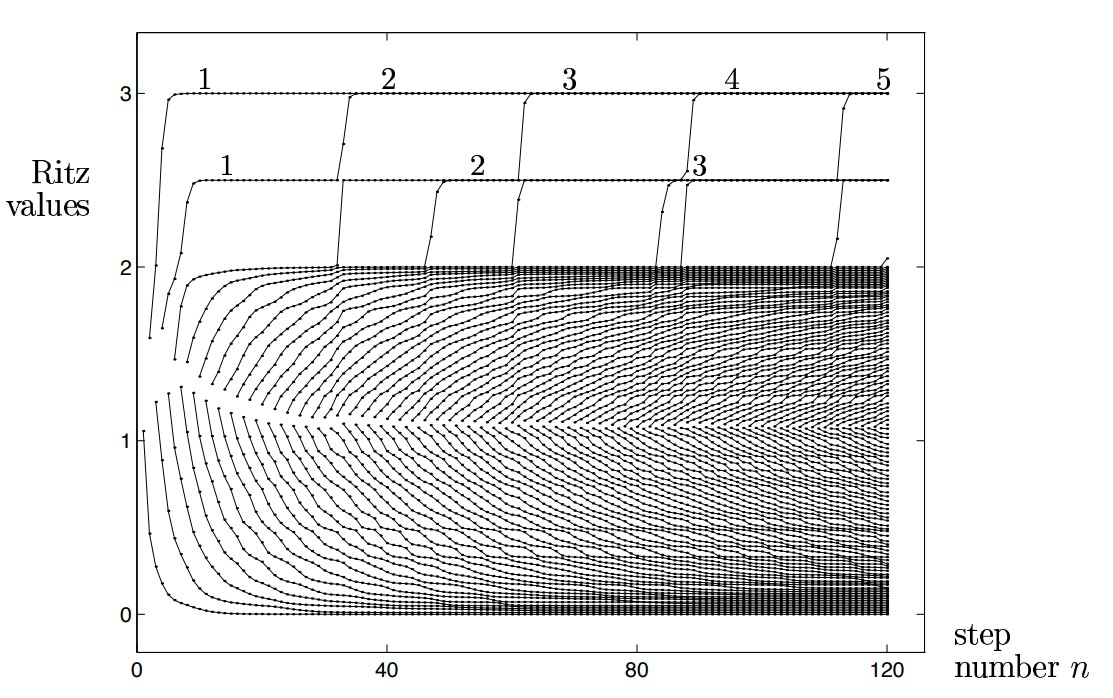
\includegraphics[scale=0.4]{Lanczos-Repeated-Eigenvalues.jpg}
    \caption{Thuật toán Lanczos được thực hiện 120 bước, các số trong hình thể hiện số bội của giá trị Ritz, có 4 giá trị Ritz "ma" tương ứng với giá tri riêng 3.0, 2 giá trị Ritz "ma" ứng với giá trị riêng 2.5 \cite{trefethen1997numerical}}

    \label{fig:Lanczos-Repeated-Eigenvalues}
\end{figure}

Hệ quả của hiện tượng này là chúng ta không thể tin tưởng vào số bội của các giá trị riêng của ma trận $A$ trong quá trình ước lượng sử dụng thuật toán lặp Lanczos.
Tuy nhiên thuật toán lặp Lanczos vẫn có thể rất hữu hiệu trong các bài toán thực tế:

\begin{itemize}
    \item PCA để giảm chiều trong phân tích dữ liệu, chúng ta chỉ cần tìm giá trị kỳ dị lớn nhất và vector kỳ dị tương ứng của ma trận $A$.
    \item Một cách tiếp cận chuẩn tắc là áp dụng thuật toán lặp Lanczos vào ma trận $A^T A$ và $A A^T$ mà không tính hai tích trên một cách rõ ràng, sử dụng các vector Ritz để xác định các vector kỳ dị.
\end{itemize}


\section{Thuật toán GMRES}

\subsection{Giới thiệu thuật toán GMRES} \label{GMRES-Introduction}

Phương pháp GMRES áp dụng cho hệ phương trình $Ax=b$ có ma trận $A$ là ma trận không kỳ dị. Ta gọi nghiệm chính xác của bài toán là $x^* = A^{-1}b$. Ý tưởng của thuật toán GMRES khá đơn giản, tại bước thứ $n$, ta xác định một vector $x_n \in \mathcal{K}_n$ làm cực tiểu hóa phần dư $r_n = b - A x_n$. Hay nói theo cách khác chúng ta đang tìm $x_n$ giải một bài toán cực tiểu hóa như ở hình \ref{fig:GMRES-LS}



Ta áp dụng công thức
\begin{algorithm}[h!]
    \hspace*{\algorithmicindent} \textbf{Input:} {Ma trận $A \in \mathbb{R}^{m \times m}$, vector $b \in \mathbb{R}^m$, chuẩn phần dư $\epsilon$ cho phép} \\
    \hspace*{\algorithmicindent} \textbf{Output:} {$x_n \in \mathbb{R}^m$}
    \caption{Các bước cơ bản thuật toán GMRES}\label{alg:GMRES}
    \begin{algorithmic}
        \State{Gán $q_1 \leftarrow b/\lVert b \rVert$}
        \For {$n=1,2,3,\dots$}
            \State {Thực hiện bước thứ n của thuật toán \ref{alg:Arnoldi} }
            \State {Tìm $y$ để cực tiểu hóa $\lVert \beta e_1 - \widetilde{H}_n y \rVert_2=\lVert r_n \rVert_2$}
            \State {$x_n \leftarrow Q_n y$}
        \EndFor
    \end{algorithmic}
\end{algorithm}

\begin{figure}[h!] \centering

    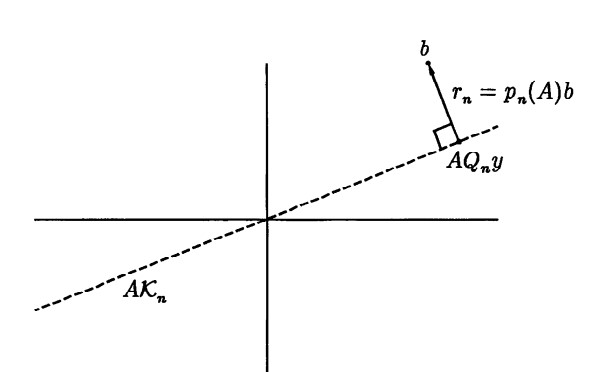
\includegraphics[scale=0.8]{GMRES-LS.jpg}
    \caption{Tìm một vector trong không gian $A \mathcal{K}_n$ \\ sao cho khoảng cách từ điểm này đến vector b nhỏ nhất}

    \label{fig:GMRES-LS}
\end{figure}

Ta xét ma trận Krylov $K_n = \begin{bmatrix} b, Ab, A^2b, \dots, A^{n-1}b \end{bmatrix}$, vì vậy:

\begin{equation}
    A K_n = \begin{bmatrix} Ab, A^2b, A^3b, \dots, A^nb \end{bmatrix}
\end{equation}

Bài toán của chúng ta là tìm một vector $c \in \mathbb{R}^n$ sao cho:

\begin{equation} \label{eq:GMRES-LS-c}
    c = \underset{c \in \mathbb{R}^{n}}{\mathrm{argmin}} \lVert b - AK_n c \rVert
\end{equation}

Với $\lVert \thickspace \rVert$ mặc định là $\lVert \thickspace \rVert_2$. Ta có thể sử dụng phân tích QR với ma trận $AK_n$. Khi đã tìm được $c$ là nghiệm của bài toán cực tiểu hóa \ref{eq:GMRES-LS-c}, $x_n=K_n c$. Nhưng bài toán trên là một bài toán không ổn định (do khi $n$ lớn ma trận $K_n$ rất gần với một ma trận kỳ dị), nên chúng ta sẽ sử dụng thuật toán lặp Arnoldi được miêu tả ở thuật toán \ref{alg:Arnoldi}
để xây dựng một dãy ma trận $Q_n$ mà các vector cột $q_1, q_2, q_3, \dots$ tạo nên cơ sở trực chuản của không gian con Krylov $\mathcal{K}_n$. Vì $x_n \in \mathcal{K}_n$, ta có thể viết $x_n = Q_n y$, bài toán cực tiểu hóa của chúng ta là tìm vector $y \in \mathbb{R}^n$, ta viết lại bài toán \ref{eq:GMRES-LS-c} dưới dạng:

\begin{equation} \label{eq:GMRES-LS-y}
    y = \underset{y \in \mathbb{R}^{n}}{\mathrm{argmin}} \lVert b - A Q_n y \rVert
\end{equation}

Ta sử dụng công thức \ref{eq:A_projection}, bài toán \ref{eq:GMRES-LS-y} có dạng:

\begin{equation}
    y = \underset{y \in \mathbb{R}^{n}}{\mathrm{argmin}} \lVert b - Q_{n+1} \widetilde{H}_n y \rVert
\end{equation}

Vì nhân một vector với một ma trận trực giao không làm thay đổi chuẩn của vector. Ta nhân các vector trong dấu $\lVert \thickspace \rVert$ với ma trận $Q_{n+1}^T$ ta được:

\begin{equation}
    y = \underset{y \in \mathbb{R}^{n}}{\mathrm{argmin}} \lVert Q_{n+1}^T b - Q_{n+1}^T Q_{n+1} \widetilde{H}_n y \rVert
\end{equation}

Trong quá trình thực hiện thuật toán lặp Arnoldi được miêu tả ở thuật toán \ref{alg:Arnoldi} để xây dựng cơ sở trực chuẩn $Q_n$ của không gian con Krylov $\mathcal{K}_n$, ta đặt $\lVert b \rVert = \beta, Q_{n+1}^T b=\lVert b \rVert e_1=\beta e_1$ với $e_1 = \begin{bmatrix}
    1 & 0 & 0 & \dots
\end{bmatrix}^T$, ta thu được dạng cuối cùng của bài toán cực tiểu hóa GMRES:

\begin{equation}
    y = \underset{y \in \mathbb{R}^{n}}{\mathrm{argmin}} \lVert \beta e_1 - \widetilde{H}_n y \rVert
\end{equation}

Tại mỗi bước $n$, ta giải bài toán cho $y$ và thu được $x_n = Q_n y$. Nhưng trong thực tế, tại mỗi bước $n$ ta không cần giải tường minh $y$ mà chỉ cần tính phần dư $\lVert \beta e_1 - \widetilde{H}_n y \rVert$, nếu phần dư này đã đủ nhỏ hơn một ngưỡng cho trước, ta sẽ dừng tại bước $n$ hiện tại và tính $x_n$. Nếu phần dư đủ nhỏ ta thực hiện bước $n+1$. Chi tiết cách tính phần dư tại mỗi bước sẽ được trình bày chi tiết ở mục sau.

Các bước cơ bản của thuật toán GMRES được trình bày ở thuật toán \ref{alg:GMRES}

Thuật toán GMRES cũng giải một bài toán xấp xỉ đa thức. Ta xét nghiệm $x_n$, tại bước $n$, vì $x_n \in \mathcal{K}_n$ nên ta có thể viết:

\begin{equation}
    x_n = c_0 b + c_1 A b + c_2 A^b + \dots + c_{n-1}A^{n-1}b=(c_0 + c_1 A + c_2 A^2 + \dots + c_{n-1} A^{n-1})b
\end{equation}

Ta đặt:

\begin{equation}
    q(z) = c_0 + c_1 z + c_2 z^2 + \dots + c_{n-1}z^{n-1}
\end{equation}

Như vậy, nghiệm tại bước thứ $n$ có thể viết dưới dạng đa thức:

\begin{equation}
    x_n = q(A)b
\end{equation}

$z(z)$ là một đa thức có bậc tối đa bằng $n-1$ với các vector hệ số $c$. Phần dư tương ứng $r_n=b - Ax_n=(I - Aq(A))b$, ta đặt đa thức $p_n(z) = 1 - z q(z)$. Như vậy ta thu được:

\begin{equation} \label{eq:Polynomial-Approximation}
    r_n = p_n(A)b
\end{equation}

Thuật toán GMRES tại mỗi bước tìm một đa thức $p_n \in P_n$ với $P_n$ là:

\begin{equation}
    P_n = \lbrace \text{là tập các đa thức có bậc } \leq n \text{ với } p(0)=1 \rbrace
\end{equation}

sao cho $p_n$ làm cực tiểu hóa phần dư (tìm vector hệ số $c$ của $p_n$):

\begin{equation} \label{eq:Find-Polynomial}
    p_n = \underset{p_n \in P_n}{\mathrm{argmin}} \lVert p_n(A)b \rVert
\end{equation}

Thuật toán GMRES cũng thỏa mãn một số tính chất bất biến như thuật toán lặp Arnoldi

\begin{dl}
    Thuật toán GMRES áp dụng cho một ma trận $A \in \mathbb{R}^{m \times m}$ thỏa mãn các tính chất sau:

    \begin{itemize}
        \item \textbf{Bất biến co dãn:} Nếu ma trận $A$ thay đổi thành $\sigma A$ với một số $\sigma \in \mathbb{R}$, và $b$ thay đổi thành $\sigma b$ thì phần dư $\lbrace r_n \rbrace$ thay đổi thành $\lbrace \sigma r_n \rbrace$.
        \item \textbf{Bất biến dưới phép biến đổi tương đương trực giao:} Nếu ma trận $A$ thay đổi thành $A A U^T$ với một ma trận $U$ trực giao bất kỳ, và $b$ thay đổi thành $Ub$, thì phần dư $\lbrace r_n \rbrace$ thay đổi thành $\lbrace U r_n \rbrace$.
    \end{itemize}
\end{dl}

Thuật toán GMRES không có tính chất bất biến tịnh tiến như thuật toán lặp Arnoldi, vì điều kiện chuẩn hóa $p(0)=1$ liên quan đến sự phụ thuộc quá trình tịnh tiến. Sự thay đổi của $\lbrace r_n \rbrace$ theo phép tịnh tiến phụ thuộc nhiều vào lựa chọn điểm gốc

\subsection{Chi tiết thực hiện thuật toán GMRES}

Một phương pháp tiêu chuẩn để giải bài toán cực tiểu hóa $y = \underset{y \in \mathbb{R}^{n}}{\mathrm{argmin}} \lVert \beta e_1 - \widetilde{H}_n y \rVert$ là phân tích ma trận $\widetilde{H}_n$ thành một một ma trận trực giao $G^T$ có kích thước $(n+1) \times (n+1)$ nhân với một ma trận tam giác trên $R$ có kích thước $(n+1) \times n$ (một ma trận mà khối $(n \times n)$ phía trên là ma trận tam giác trên và hàng cuối cùng là một vector hàng 0):

\begin{equation} \label{eq:Givens-Apply}
    \lVert r_n \rVert = \lVert G(\beta e_1 - \widetilde{H}_n y) \rVert = \lVert \beta G e_1 - R_n y \rVert
\end{equation}


Ta có thể sử dụng phương pháp phân tích Householder nhưng trong trường hợp với cấu trúc ma trận Hessenberg $\widetilde{H}_n$, ta sẽ sử dụng phương pháp ma trận quay Givens để đưa ma trận $\widetilde{H}_n$ về dạng ma trận tam giác trên.
Phương pháp ma trận quay Givens (phép quay Givens) là một phương pháp hiệu quả để tạo ra các phần tử 0 bằng cách nhân ma trận với một ma trận trực giao hạng thấp. Ví dụ: ta muốn biến đổi một ma trận $A$ thành một ma trận tam giác trên $R$ trong phân tích QR.
Ma trận Givens được ký hiệu là $G(i, k, \theta) \in \mathbb{R}^{n \times n}$ được cho bởi công thức:

\begin{equation} \label{eq:Givens-Rotation-Matrix}
    G(i, k, \theta) = \begin{bmatrix} 1 & 0 & \dots & 0 & \dots & 0 & \dots & 0 \\
                                    0 & 1 & \dots & 0 & \dots & 0 & \dots & 0 \\
                                    \vdots & \thickspace & \ddots & \thickspace & \thickspace & \thickspace & \thickspace \\
                                    0 & \thickspace & \space & c & \thickspace & s & \thickspace & 0 \\
                                    \vdots \\
                                    0 & \thickspace & \space & -s & \thickspace & c & \thickspace & 0 \\
                                    \vdots \\
                                    0 & \dots & \thickspace & \thickspace & \thickspace & \thickspace & \space & 1    \end{bmatrix}
\end{equation}

với $c = \cos(\theta), s = \sin(\theta)$. Ma trận trên tác động lên vector $x: y=G(i, k, \theta)x$

\begin{equation} \label{eq:Rotation-Result}
    y_j = \begin{cases}
        \cos(\theta) x_i + \sin(\theta) x_k, \thickspace j = i \\
        -\sin(\theta) x_i + \cos(\theta) x_k, \thickspace j = k \\
        x_j, \thickspace j \neq i, k
    \end{cases}
\end{equation}

Phép quay chọn:

\begin{equation}
    \begin{cases}
        \cos(\theta) = \dfrac{x_i}{\sqrt{x_i^2 + x_k^2}} \\
        \sin(\theta) = \dfrac{x_k}{\sqrt{x_i^2 + x_k^2}}
    \end{cases}
\end{equation}

Vì vậy $y_k = 0$. Ví dụ trong không gian hai chiều, ta quay một vector $x$ thành một vector $y$ nằm trên trục hoành. Phép quay bảo toàn độ dài của vector $x$.

Ví dụ ta xét ma trận $\widetilde{H}_4$:

\begin{equation}
    \widetilde{H}_4 = \begin{bmatrix} h_{11} & h_{12} & h_{13} & h_{14} \\
                                    h_{21} & h_{22} & h_{23} & h_{24} \\
                                    0 & h_{32} & h_{33} & h_{34} \\
                                    0 & 0 & h_{43} & h_{44} \\
                                    0 & 0 & 0 & h_{54}  \end{bmatrix}
\end{equation}

Ta áp dụng các phép quay Givens thu được:

\begin{equation}
    G(1, 2, \theta_1) \widetilde{H}_4 = \begin{bmatrix} r_{11}^{'} & r_{12}^{'} & r_{13}^{'} & r_{14}^{'} \\
        0 & r_{22}^{'} & r_{23}^{'} & r_{24}^{'} \\
        0 & h_{32} & h_{33} & h_{34} \\
        0 & 0 & h_{43} & h_{44} \\
        0 & 0 & 0 & h_{54}  \end{bmatrix}
\end{equation}

\begin{equation}
    G(2, 3, \theta_2)G(1, 2, \theta_1) \widetilde{H}_4 = \begin{bmatrix} r_{11}^{'} & r_{12}^{'} & r_{13}^{'} & r_{14}^{'} \\
        0 & r_{22}^{''} & r_{23}^{''} & r_{24}^{''} \\
        0 & 0 & r_{33}^{'} & r_{34}^{'} \\
        0 & 0 & h_{43} & h_{44} \\
        0 & 0 & 0 & h_{54}  \end{bmatrix}
\end{equation}

\begin{equation}
    G(3, 4, \theta_3)G(2, 3, \theta_2)G(1, 2, \theta_1) \widetilde{H}_4 = \begin{bmatrix} r_{11}^{'} & r_{12}^{'} & r_{13}^{'} & r_{14}^{'} \\
        0 & r_{22}^{''} & r_{23}^{''} & r_{24}^{''} \\
        0 & 0 & r_{33}^{''} & r_{34}^{''} \\
        0 & 0 & 0 & r_{44}^{'} \\
        0 & 0 & 0 & h_{54}  \end{bmatrix}
\end{equation}

\begin{equation}
    G(4, 5, \theta_4)G(3, 4, \theta_3)G(2, 3, \theta_2)G(1, 2, \theta_1) \widetilde{H}_4 = \begin{bmatrix} r_{11}^{'} & r_{12}^{'} & r_{13}^{'} & r_{14}^{'} \\
        0 & r_{22}^{''} & r_{23}^{''} & r_{24}^{''} \\
        0 & 0 & r_{33}^{''} & r_{34}^{''} \\
        0 & 0 & 0 & r_{44}^{''} \\
        0 & 0 & 0 & 0  \end{bmatrix}
\end{equation}

Tại mỗi bước $n$, chúng ta chỉ áp dụng $G(n-1, n, \theta_{n-1})G(n-2, n-1, \theta_{n-2})\dots G(1, 2, \theta_1)$ vào cột cuối cùng của ma trận $\widetilde{H}_n$, sau đó ta xác định ma trận quay $G(n, n+1, \theta_{n})$ và áp dụng vào kết quả của bước trên bởi vì $G(n, n+1, \theta_{n})$ không tác dụng lên các cột phía trước cột hiện tại (cột thứ $n$ của $\widetilde{H}_n$). Chi phí để thực hiện phân tích QR tại mỗi bước $n$ là:

\begin{itemize}
    \item Cần áp dụng $n$ ma trận quay vào cột thứ $n$ của ma trận $\widetilde{H}_n$
    \item Từ công thức \ref{eq:Rotation-Result}, mỗi phép quay ta cần 6 phép tính (4 phép nhân, 2 phép cộng)
\end{itemize}

Vì vậy, tại mỗi bước $n$ của thuật toán GMRES, ta cần $6n$ phép tính. Số phép tính tích lũy cần để phân tích QR cho ma trận $\widetilde{H}_n$ tính từ cột đầu tiên đến cột thứ $n=6(1+2+3+\dots+n)=6\dfrac{n(n+1)}{2}\sim \mathcal{O}(n^2)$
phép tính.

Một vấn đề nữa là chúng ta cần tìm $y$ và tính $\lVert r_n \rVert$ tại bước lặp thứ $n$.
Để tìm $y$, từ công thức \ref{eq:Givens-Apply}, ta giải $y$ bằng giải hệ phương trình lấy $n$ hàng đầu của $R_n$ và $n$ phần tử đầu của $\beta G e_1$. Đặt $\beta G e_1 = g_n$:

\begin{equation} \label{eq:GMRES-Y-Backsubstitute}
    R_n \lbrack 1:n,1:n \rbrack y = g_n \lbrack 1:n \rbrack
\end{equation}

Đây là hệ phương trình gồm $n$ phương trình và $n$ ẩn, $y$ có thể giải bằng phép thế ngược do block phía trên của $R_n$ là ma trận tam giác trên.

Để tính $\lVert r_n \rvert$, ta nhận thấy $r_n=g_n - R_n y$ có $n$ thành phần đầu bằng 0 do nghiệm $y$ thỏa mãn phương trình ở công thức \ref{eq:GMRES-Y-Backsubstitute}. Mặt khác do hàng cuối của $R_n$ là vector hàng 0 nên thành phần thứ $n+1$ của phần dư $r_n$ chính bằng thành phần thứ $n+1$ của $g_n$.

\begin{md}
    Chuẩn phần dư của nghiệm $x_n$ tại bước lặp thứ $n$ bằng thành phần thứ $n+1$ của vector $g_n$ thu được bằng cách nhân phía bên trái của $\beta e_1$ với liên tiếp các phép quay Givens biến đổi ma trận $\widetilde{H}_n$ thành ma trận tam giác trên.
\end{md}

Trong thực tế, khi giải các bài toán, tại mỗi bước ta thường kiểm tra chuẩn phần dư $\lVert r_n \rVert$ trước khi giải ra nghiệm $y$. Do trước khi thực hiện thuật toán, chúng ta có một ngưỡng chuẩn phần dư cho phép dừng vòng lặp $\epsilon$. Nếu tại bước hiện tại $n$, ta kiểm tra chuẩn phần dư $\lVert r_n \rvert$, nếu $\lbrack r_n \rbrack < \epsilon$ thì ta dừng vòng lặp, giải $y$ và tính $x_n=Q_n y$. Nếu không ta chuyển sang bước thứ $n+1$.

Từ các lập luận trên, ta có sơ đồ mã giả chi tiết của thuật toán GMRES được miêu tả ở thuật toán \ref{alg:GMRES-Detailed}:

\begin{algorithm}[h!]
    \caption{Các bước chi tiết thuật toán GMRES}\label{alg:GMRES-Detailed}
    \hspace*{\algorithmicindent} \textbf{Input:} {Ma trận $A \in \mathbb{R}^{m \times m}$ không kỳ dị, vector $b \in \mathbb{R}^m$, chuẩn phần dư $\epsilon$ cho phép} \\
    \hspace*{\algorithmicindent} \textbf{Output:} {$x_n \in \mathbb{R}^m$}
    \begin{algorithmic}
        \State{$q_1 \leftarrow b/\lVert b \rVert$}
        \State{$\beta \leftarrow \lVert b \rVert$}
        \State{$g_0 \leftarrow \beta$}
        \For {$n=1,2,3,\dots$}
            \State {Thực hiện bước thứ n của thuật toán \ref{alg:Arnoldi} thu được $q_{n+1}$ và cột thứ $n$ của ma trận $\widetilde{H}_n$}
            \State {Tính $G(n-1, n, \theta_{n-1})G(n-2, n-1, \theta_{n-2})\dots G(1, 2, \theta_1)$ vào cột cuối cùng của ma trận $\widetilde{H}_n$}
            \State {Tính ma trận quay $G(n, n+1, \theta_n)$ từ kết quả của bước trên và áp dụng vào kết quả này}
            \State {$g_{n-1} \leftarrow \begin{bmatrix} g_{n-1} & 0 \end{bmatrix}$}
            \State {$g_n \leftarrow G(n, n+1, \theta_n) g_{n-1}$}
            \If {Nếu thành phần thứ $n+1$ của $g_n < \epsilon$ }
                \State {Giải $y$ từ phương trình $R_n \lbrack 1:n,1:n \rbrack y = g_n \lbrack 1:n \rbrack$}
                \State {$x_n \leftarrow Q_n y$}
                \State \Return $x_n$
                \State {break}
            \EndIf
        \EndFor
    \end{algorithmic}
\end{algorithm}

\subsection{Một số đặc điểm của thuật toán GMRES} \label{GMRES-Characteristic}


\subsubsection{Chi phí bộ nhớ} \label{GMRES-Storage}

Thuật toán GMRES yêu cầu một lượng lớn bộ nhớ và trở nên rất đắt khi số bước lặp cao.
Yêu cầu về bộ nhớ cơ bản là lưu các vector $b, x \in \mathbb{R}^{m}$ và ma trận $A \in \mathbb{R}^{m \times m}$. Nếu $A$ là ma trận thưa, mỗi hàng có $l$ phần tử khác 0 thì yêu cầu về bộ nhớ cần lưu $(l+2)m$ số thực để tạo bài toán. Thuật toán GMRES cần phải lưu tất cả các vector $q_1, q_2, \dots, q_n$. Từng vector $q_i \in \mathbb{R}^{m}, i=1\dots n$, vì vậy cần chi phí bộ nhớ là $mn$ số thực.
Ngoài ra ta cần giải bài toán cực tiểu hóa, ta thu được $y \in \mathbb{R}^n$, tại bước lặp thứ $n$ $x_n = Q_n y$ (nếu thỏa mãn điều kiện hội tụ là $\lVert r_n \rVert < \epsilon$), ta cần lưu $n$ số thực cho $y$.
Chúng ta cũng cần lưu ma trận $\widetilde{H}_n$, thực tế chúng ta lưu ma trận $R_n \in \mathbb{R}^{(n+1) \times n}$ với chi phí $\dfrac{n^2 + n}{2}$.
Cuối cùng chúng ta cần lưu các ma trận quay Givens, mỗi ma trận quay cần lưu hai số $\sin$ và $\cos$. Tại bước thứ $n$, cần lưu $n$ ma trận quay Givens từ $\sin(\theta_1),\dots, \sin(\theta_n)$ và $\cos(\theta_1),\dots,\cos(\theta_n)$ như vậy chi phí là $2n$.
Tổng hợp lại chi phí bộ nhớ cho thuật toán GMRES tại bước thứ $n$ là: $(l+2)m + mn + n + \dfrac{n^2 + n}{2} + 2n$.

\subsubsection{Chi phí tính toán} \label{GMRES-Computation-Cost}

Tại mỗi bước $n$, của thuật toán GMRES, ta cần thực hiện các công việc:

\begin{itemize}
    \item Thực hiện thuật toán Arnoldi để thu được vector $q_{n+1}$ và cột thứ $n$ của ma trận $\widetilde{H}_n$. Bước này chi phí là: \begin{itemize}
        \item Tính $Aq_n$ cần $m(2m-1)$ phép tính
        \item $n$ bước, mỗi bước gồm 1 phép nhân vô hướng ($h_{j,n} \leftarrow q_j^Tv$) cần $2m-1$ phép tính và một bước nhân 1 số ($h_{j,n}q_j$) với một vector cần $m$ phép tính và một bước trừ hai vector cần $m$ phép tính ($v \leftarrow v - h_{j,n}q_j$). Như vậy bước này cần $n(4m-1)$ phép tính.
        \item Một bước tính chuẩn ($h_{n+1,n} \leftarrow \lVert v \rVert$) cần $2m$ phép tính.
        \item Một bước chuẩn hóa ($q_{n+1} \leftarrow v/h_{n+1,n}$) cần $m$ phép tính.
    \end{itemize}
    Như vậy số phép tính để thực hiện thuật toán Arnoldi cần $m(2m-1) + n(4m-1) + 2m + m=m(2m-1) + n(4m-1)+ 3m=2m^2+4mn+2m-n$.
    \item Bước áp dụng phép quay Givens cho cột thứ $n$ của ma trận $\widetilde{H}_n$ gồm $6n+10$ ($10$ là số phép tính để tính $\sin(\theta_n)$ và $\cos(\theta_n)$).
    \item Bước cập nhật $g_n \leftarrow G(n, n+1, \theta_n)g_{n-1}$ cần 6 phép tính
\end{itemize}

Như vậy tại bước thứ $n$ của thuật toán GMRES ta cần số phép tính là: $2m^2+4mn+2m-n + 6n+10 + 6=2m^2+4mn+2m+5n+16$ phép tính.

Nếu giả sử tại bước $n$, điều kiện hội tụ đã thỏa mãn $\lVert r_n \rVert < \epsilon$, ta cần thêm bước giải $y$ bằng phép thế ngược. Để giải hệ ở phương trình \ref{eq:GMRES-Y-Backsubstitute}, tại bước thế ngược thứ $k, k=1,2,\dots,n$, ta cần số phép tính:
\begin{itemize}
    \item 1 phép chia
    \item $k-1$ phép nhân
    \item $k-1$ phép trừ
\end{itemize}

Vậy số bước cần để giải hệ phương trình \ref{eq:GMRES-Y-Backsubstitute} là $n + 2\lbrack 0 + 1 + \dots + (k-1) + \dots + (n-1)\rbrack=n+(n-1)n=n^2$ phép tính

Ngoài ra ta cần tính $x_n = Q_n y$ cần $m(2n-1)$ phép tính

Ta tổng hợp số phép tính tích lũy từ khi bắt đầu đến khi nhận được lời giải sử dụng thuật toán GMRES là: $2m^2 n + 4m\dfrac{n(n+1)}{2}+2mn + 5\dfrac{n(n+1)}{2}+16n+n^2+m(2n-1)=2m^2 n + 2mn^2+4mn+3.5n^2+3m+15n+2.5 \sim \mathcal{O}(2m^2n+ 2mn^2)$

Ta thấy chi phí tính toán là một nhược điểm lớn của GMRES, do tại mỗi bước $n$, chi phí tính toán phần thực hiện thuật toán lặp Arnoldi phụ thuộc vào $n$ ($2m^2+4mn+2m+5n+15$) khiến cho $n$ càng lớn thì chi phí tính toán càng lớn, bước sau chi phí tính toán nhiều hơn bước trước. Đây là vấn đề cần được cải thiện đối với thuật toán GMRES.

\subsubsection{Sự hội tụ của thuật toán GMRES} \label{GMRES-Convergence}

Ta nhận thấy có hai quan sát với phần dư của thuật toán GMRES:

\begin{itemize}
    \item $ \lVert r_{n+1} \rVert \leq \lVert r_{n} \rVert $. Lý do là vì $\lVert r_n \rVert$ nhỏ nhất có thể trong không gian con Krylov thứ $n$ $\mathcal{K}_n$, khi mở rộng không gian con Krylov $\mathcal{K}_n$ sang $\mathcal{K}_{n+1}$, chuẩn phần dư chỉ có thể giảm hoặc tệ nhất là chuẩn phần dư không thay đổi.
    \item Mặt khác sau khi thực hiện $m$ bước lặp, quá trình phải hội tụ hay $\lVert r_m \rVert=0$. $\lVert r_m \rVert = 0$ sẽ xảy ra khi $\mathcal{K}_m = \mathbb{R}^m$ và trong trường hợp đặc biệt nếu vector $b \in \mathcal{K}_n$ với một số $n < m$, thì sự hội tụ sẽ xảy ra sớm hơn. $\lVert r_m \rVert = 0$ chỉ có ý nghĩa về mặt lý thuyết của thuật toán GMRES nhưng không có nhiều ý nghĩa về mặt thực tiễn, chúng ta mong rằng GMRES sẽ hội tụ sau $n$ bước nhỏ hơn rất nhiều so với $m$.
\end{itemize}

Để thu được nhiều thông tin hữu ích hơn về quá trình hội tụ của thuật toán GMRES, ta phải sử dụng bài toán xấp xỉ đa thức đã được đề cập ở mục \ref{GMRES-Introduction}. Từ công thức \ref{eq:Polynomial-Approximation}, ta biết rằng: $\lVert r_n \rVert=\lVert p_n(A)b \rVert \leq \lVert p_n(A) \rVert \lVert b \rVert$. Ngoại trừ trường hợp $b$ có cấu trúc đặc biệt liên quan đến ma trận $A$ thì nhân tố quan trọng xác định $ \lVert r_n \rVert$ là $\lVert p_n(A) \rVert$. Bất đẳng thức xác định tốc độ hội tụ của thuật toán GMRES là:

\begin{equation} \label{eq:GMRES-Convergence-Rate}
    \dfrac{\lVert r_n \rVert}{\lVert b \rVert} \leq \inf_{p_n \in P_n} \lVert p_n(A) \rVert
\end{equation}

Ta cần phân tích với một ma trận $A$ và một số $n$ cho trước thì $\lVert p_n(A) \rVert$ có thể nhỏ bao nhiêu. Cách tiếp cận tiêu chuẩn là tìm một đa thức $p(z)$ sao cho $p(z)$ càng nhỏ càng tốt trên tập phổ của ma trận $A$ $\Lambda(A)$ và thỏa mãn $p(0)=1$. Ta giả sử ma trận $A$ là ma trận chéo hóa được, thỏa mãn $A=V\Lambda V^{-1}$ với $V$ là ma trận không kỳ dị và $\Lambda$ là ma trận đường chéo. Ta có bất đẳng thức:

\begin{equation}
    \lVert p_n(A) \rVert \leq \lVert V \rVert \lVert p_n(\Lambda) \rVert \lVert V^{-1} \rVert = \dfrac{\max(\sigma(V))}{\min(\sigma(V))} \lVert p_n(\Lambda) \rVert = \kappa(V) \lVert p_n(\Lambda) \rVert
\end{equation}

Từ công thức trên và công thức \ref{eq:GMRES-Convergence-Rate}, ta đi đến định lý:

\begin{dl} \label{dl:GMRES-Convergence-Rate}
    Tại bước thứ $n$ của thuật toán GMRES, phần dư $r_n$ thỏa mãn:
    \begin{equation}
        \dfrac{\lVert r_n \rVert}{\lVert b \rVert} \leq \inf_{p_n \in P_n} \lVert p_n(A) \rVert \leq \kappa(V) \inf_{p_n \in P_n} \lVert p_n \rVert_{\Lambda(A)}
    \end{equation}
    với $\Lambda(A)$ là tập các giá trị riêng của ma trận $A$, $V$ là ma trận không kỳ dị của các vector riêng của ma trận $A$ (giả sử ma trận $A$ chéo hóa được), $\kappa(V)$ là số điều kiện của ma trận $V$ và $\lVert p_n \rVert_{\Lambda(A)}=\underset{s \in \Lambda(A)}{\sup} \lvert p_n(s) \rvert$
\end{dl}

Ý nghĩa của định lý \ref{dl:GMRES-Convergence-Rate} là nếu ma trận $A$ có số điều kiện của ma trận $V$ là $\kappa(V)$ không quá lớn và một đa thức thuộc tập $P_n$ được tìm thấy mà độ lớn của nó trên phổ của ma trận $A$ là $\Lambda(A)$ giảm nhanh theo $n$ thì thuật toán GMRES hội tụ nhanh.

Thuật toán GMRES sẽ hội tụ khi ta thực hiện số bước lặp bằng với số giá trị riêng riêng biệt của ma trận $A$. Sự hội tụ sẽ phụ thuộc vào cấu trúc các giá trị riêng của ma trận $A$ được phân bố thế nào.
Từ bài toán tìm đa thức $p_n \in P_n$ được nêu ở công thức \ref{eq:Find-Polynomial}, ta đặt đa thức $p_n$ có dạng:

\begin{equation}
    p_n(s) = 1 - \sum_{i=1}^n c_i s^i
\end{equation}

Trong quá trình giải bài toán cực tiểu bằng việc tìm đa thức mà giá trị của nó nhỏ trên phổ của ma trận $A$ hay giá trị của nó nhỏ với mọi giá trị riêng của ma trận $A$. Trong trường hợp đặc biệt nếu $n$ lớn hơn số giá trị riêng của ma trận $A$ thì đa thức này sẽ bằng 0 tại mọi giá trị riêng của ma trận $A$ và thuộc $P_n$.
Nhưng đôi khi chúng ta chỉ hy vọng tìm được một đa thức mà có giá trị đủ nhỏ tại tất cả các giá trị riêng. Việc tìm đa thức sẽ càng dễ hơn nếu các giá trị riêng phân thành các nhóm mà mỗi nhóm các giá trị riêng nằm sát nhau và khó hơn nếu các giá trị riêng có các giá trị riêng biệt và nằm xa nhau. Và việc phân bố các giá trị riêng của ma trận $A$ có mối quan hệ mật thiết với số điều kiện của ma trận $A$.

Nếu $\kappa(V)$ nhỏ thì ta có hai trường hợp:
\begin{itemize}
    \item Nếu ma trận $A$ đối xứng xác định dấu dương thì thuật toán GMRES cần $O(\sqrt{\kappa})$ bước để hội tụ.
    \item Nếu ma trận $A$ không xác định dấu thì thuật toán GMRES cần $O(\kappa)$ bước để hội tụ.
\end{itemize}

Nếu ma trận $A$ là một ma trận không chéo hóa được, nếu $n^{*}$ là số chiều của \textit{không gian bất biến tổng quát nhỏ nhất} chứ vector $b$, thuật toán GMRES sẽ dừng sau đúng $n^{*}$ bước. Một không gian $\mathcal{S}$ được gọi là \textit{không gian con bất biến tổng quát} nếu $v \in \mathcal{S} \Rightarrow A^{n}v \in \mathcal{S} \thickspace \forall n \geq 0$ 

Nếu ma trận $A=VJV^{-1}$ với ma trận $J$ là một ma trận có dạng chuẩn Jordan thì:

\begin{equation}
    \lVert p_n(A) \rVert \leq \lVert V \rVert \lVert p_n(J) \rVert \lVert V^{-1} \rVert=\dfrac{\max(\sigma(V))}{\min(\sigma(V))} \lVert p_n(J) \rVert = \kappa(V) \lVert p_n(J) \rVert
\end{equation}

và:

\begin{equation}
    \dfrac{\lVert r_n \rVert}{\lVert b \rVert} \leq \inf_{p_n \in P_n} \lVert p_n(A) \rVert \leq \kappa(V) \inf_{p_n \in P_n} \lVert p_n(J) \rVert
\end{equation}

Để đánh giá $\inf_{p_n \in P_n} \lVert p_n(J) \rVert$ khá phức tạp, giá trị này được phân tích rất kỹ trong \cite{tichy2005worst}.

\textbf{Ví dụ:} Một ma trận $A$ có kích thước $200\times 200$ mà từng phần từ của nó độc lập và được lấy mẫu từ phân bố chuẩn $\mathcal{N}\Bigg(2;\Big(\dfrac{0.5}{\sqrt{200}} \Big)^2 \Bigg)$

\begin{figure}[h!] \centering

    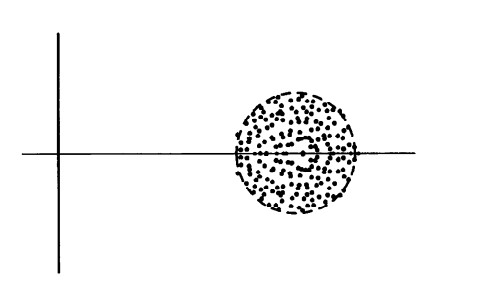
\includegraphics[scale=1.0]{A-Eigenvalues.jpg}
    \caption{Các giá trị riêng của ma trận $A$ ở ví dụ trên, đường tròn nét đứt là đường tròn có tâm $(0; 2)$ và bán kinh $R=\dfrac{1}{2}$ \cite{trefethen1997numerical}}

    \label{fig:A-Eigenvalues}
\end{figure}

\begin{figure}[h!] \centering

    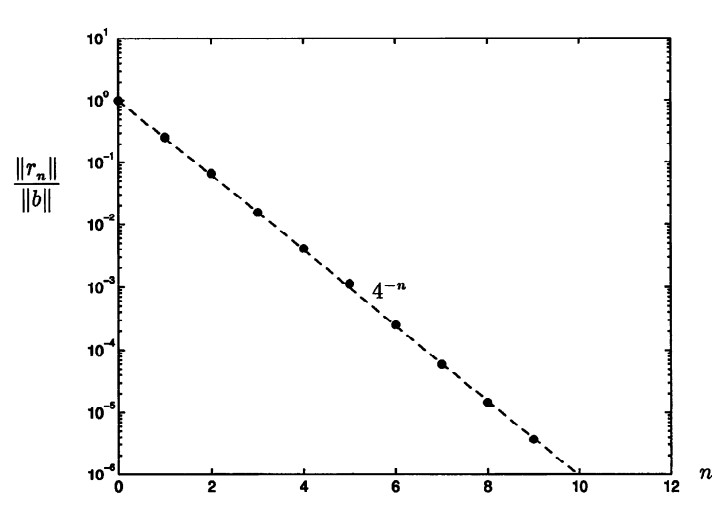
\includegraphics[scale=0.6]{GMRES-Convergence-Curve.jpg}
    \caption{Đường cong hội tụ $\dfrac{\lVert r_n \rVert}{\lVert b \rVert} $ theo thuật toán GMRES của ma trận $A$ \cite{trefethen1997numerical}}

    \label{fig:GMRES-Convergence-Curve}
\end{figure}

Hình \ref{fig:A-Eigenvalues} thể hiện các giá trị riêng của ma trận $A$, một tập các điểm được phân bố đều trong một chiếc đĩa bán kính $R=\dfrac{1}{2}$ và tâm $(0;2)$. Hình \ref{GMRES-Convergence} đường cong hội tụ khi thực hiện thuật toán GMRES giải hệ phương trình $Ax=b$ với $b=\begin{bmatrix} 1 & 1 \dots & 1 \end{bmatrix}^T$. Sự hội tụ trong trường hợp này bằng $4^{-n}$. Ta có phổ của ma trận $A$ là $\Lambda(A)$ nằm trong một chiếc đĩa được miêu tả ở trên. $\lVert p_n(A) \rVert $ được cực tiểu hóa với lựa chọn $p_n(s)=(1-s/2)^n$, ta có $\lVert p_n(A) \rVert = \lVert (I - A/2)^n \rVert \approx 4^{-n}$. Ma trận $A$ là ma trận có điều kiện tốt với số điều kiện $\kappa(A) \approx 2.03$

\textbf{Ví dụ:} Cho trước các giá trị riêng (chấm đỏ) và các đa thức $p_n$ (các đường cong màu xanh) được chọn được biểu diễn trên các hình \ref{fig:Convergence-Behavior-1} và hình \ref{fig:Convergence-Behavior-2}, phân tích sự hội tụ trong từng trường hợp

\begin{figure}[h!] \centering

    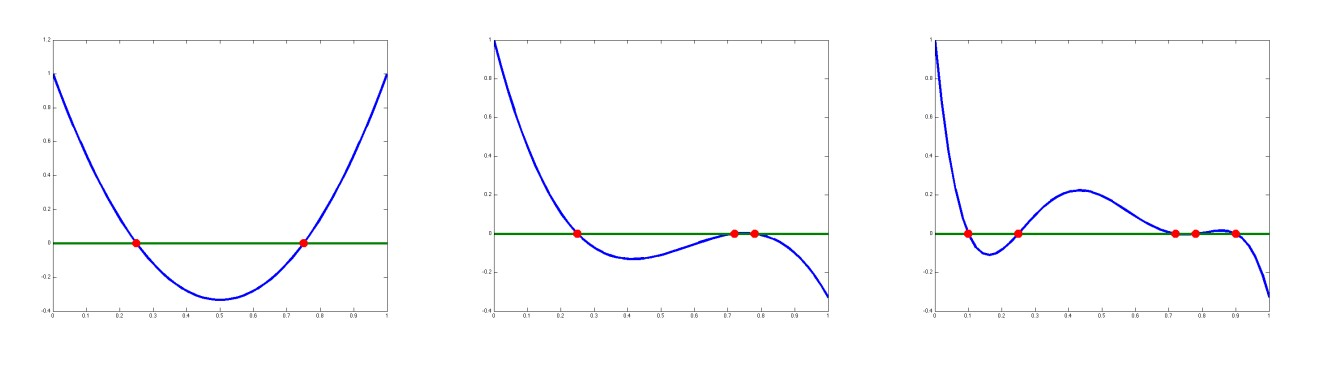
\includegraphics[scale=0.5]{Convergence-Behavior-1.jpg}
    \caption{Các ví dụ chọn đa thức tương ứng với tập các giá trị riêng của ma trận $A$}

    \label{fig:Convergence-Behavior-1}
\end{figure}

\begin{figure}[h!] \centering

    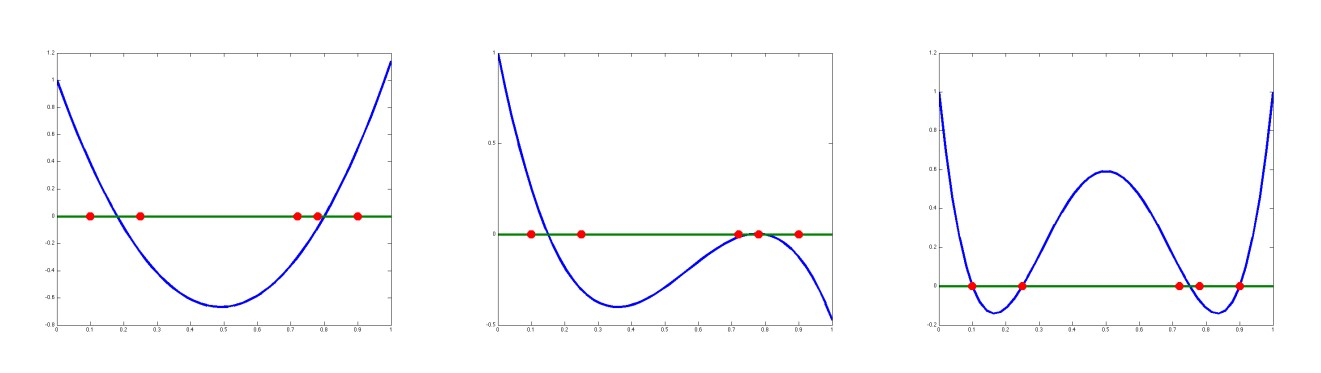
\includegraphics[scale=0.5]{Convergence-Behavior-2.jpg}
    \caption{Các ví dụ chọn đa thức tương ứng với tập các giá trị riêng của ma trận $A$}

    \label{fig:Convergence-Behavior-2}
\end{figure}

Trong hình \ref{fig:Convergence-Behavior-1}, hình đầu tiên bên trái ma trận $A$ có hai giá trị riêng, đa thức được chọn là một hàm bậc 2, đường cong này có giá trị bằng 0 tại các giá trị riêng, hình thứ 2 ma trận $A$ có 3 giá trị riêng và đa thức được chọn là một hàm bậc 3 hay hình thứ 3 ma trận $A$ có 5 giá trị riêng, tương tự đa thức được chọn là một hàm bậc 5. Trong trường hợp cả 3 hình này, phần dư đều đã về 0, thuật toán GMRES tìm được nghiệm chính xác tương ứng sau số bước lặp chính bằng số giá trị riêng của ma trận $A$.

Trong hình \ref{fig:Convergence-Behavior-2}, cả 3 hình đều biểu diễn các giá trị riêng của ma trận $A$ có 5 giá trị riêng, nhưng thể hiện các đường cong là các đa thức được chọn tại các bước lặp $n$ khác nhau. Hình đầu tiên bên trái, tại $n=2$, đa thức được chọn là hàm số bậc 2 nhưng giá trị của đa thức này tại các giá trị riêng vẫn khá lớn (chỉ nhỏ tại giá trị riêng thứ 4). Hình thứ 2 tại $n=3$, đa thức được chọn là hàm số bậc 3, giá trị của đa thức này khá nhỏ ở 3 giá trị riêng bên phải nhưng vẫn khá lớn ở 2 giá trị riêng bên trái nên phần dư tại $n=3$ vẫn khá lớn. Hình cuối cùng tại $n=4$, đa thức được chọn là hàm số bậc 4 đã có giá trị rất nhỏ tại tất cả các giá trị riêng của ma trận $A$, ta đã có thể dừng tại bước này vì phần dư đã đủ nhỏ. Tuy nhiên nếu ta thực hiện thêm bước lặp $n=5$, ta sẽ chọn được một đa thức là hàm số bậc 5 và có giá trị bằng 0 tại mọi giá trị riêng.

Từ ví dụ trên, ta xác nhận một điều. Nếu ma trận $A$ có $n$ giá trị riêng riêng biệt thì thuật toán GMRES sẽ tìm được nghiệm chính xác sau $n$ bước lặp. Nếu các giá trị riêng phân thành các nhóm gần nhau thì thuật toán GMRES sẽ cần số bước ít hơn (xấp xỉ bằng số nhóm) để đạt điều kiện hội tụ. Nếu các giá trị riêng tách biệt xa nhau, thuật toán cần nhiều bước (xấp xỉ số giá trị riêng riêng biệt) để đạt điều kiện hội tụ.

\subsection{Cải thiện thuật toán GMRES}

\subsubsection{Phương pháp khởi tạo lại}

Từ các phân tích ở mục \ref{GMRES-Characteristic}, ta thấy rằng chi phí về lưu trữ bộ nhớ và chi phí tính toán tăng theo $n$. Đây là nhược điểm rất lớn của thuật toán GMRES, vì vậy trong thực tế ta sẽ hay sử dụng phương pháp khởi tạo lại.
Ý tưởng của phương pháp này là chọn giới hạn số bước lặp $n_{\max}$. Khi $n$ đạt đến $n_{\max}$ mà thuật toán GMRES chưa hội tụ, ta tính $x_{n_{\max}}$ và bỏ tất cả các vector trực giao $q_1, q_2, \dots, q_{n_{\max}}$ chỉ giữ lại nghiệm tại bước lặp $x_{n_{\max}}$. Đặt $x_{n_{\max}}=x_0$, ta quay trở lại giải hệ phương trình:

\begin{equation} \label{eq:Restart-Equation}
    A(x - x_0) = b - A x_0 = r_0
\end{equation}

Cách giải hệ phương trình \ref{eq:Restart-Equation} hoàn toàn tương tự như trình tự đã được trình bày ở thuật toán \ref{alg:GMRES-Detailed} chỉ khác là vai trò của $b$ đã được thay bằng $r_0$ và $x_n$ được thay bằng $x_0+Q_n y$

\begin{algorithm}[h!]
    \caption{Các bước chi tiết thuật toán GMRES khởi tạo lại}\label{alg:GMRES-Restart}
    \hspace*{\algorithmicindent} \textbf{Input:} {Ma trận $A \in \mathbb{R}^{m \times m}$ không kỳ dị, vector $b \in \mathbb{R}^m$, $n_{\max}$, chuẩn phần dư $\epsilon$ cho phép} \\
    \hspace*{\algorithmicindent} \textbf{Output:} {$x_n \in \mathbb{R}^m$}
    \begin{algorithmic}
        \State{$x_0 \leftarrow 0$}
        \State{$r_0 \leftarrow b - A x_0$}
        \State{$q_1 \leftarrow r_0 / \lVert r_0 \rVert$}
        \State{$\beta \leftarrow \lVert r_0 \rVert$}
        \State{$g_0 \leftarrow \beta$}
        \For {$n=1,2,3,\dots, n_{\max}$}
            \State {Thực hiện bước thứ n của thuật toán \ref{alg:Arnoldi} thu được $q_{n+1}$ và cột thứ $n$ của ma trận $\widetilde{H}_n$}
            \State {Tính $G(n-1, n, \theta_{n-1})G(n-2, n-1, \theta_{n-2})\dots G(1, 2, \theta_1)$ vào cột cuối cùng của ma trận $\widetilde{H}_n$}
            \State {Tính ma trận quay $G(n, n+1, \theta_n)$ từ kết quả của bước trên và áp dụng vào kết quả này}
            \State {$g_{n-1} \leftarrow \begin{bmatrix} g_{n-1} & 0 \end{bmatrix}$}
            \State {$g_n \leftarrow G(n, n+1, \theta_n) g_{n-1}$}
            \If {Nếu thành phần thứ $n+1$ của $g_n < \epsilon$ }
                \State {Giải $y$ từ phương trình $R_n \lbrack 1:n,1:n \rbrack y = g_n \lbrack 1:n \rbrack$}
                \State {$x_n \leftarrow x_0 + Q_n y$}
                \State \Return $x_n$
                \State {break}
            \EndIf

            \If {$n = n_{\max}$}
                \State {Giải $y$ từ phương trình $R_{n_{\max}} \lbrack 1:n_{\max},1:n_{\max} \rbrack y = g_{n_{\max}} \lbrack 1:n_{\max} \rbrack$}
                \State {$x_{n_{\max}} \leftarrow x_0 + Q_{n_{\max}} y$}
                \State {$x_0 \leftarrow x_{n_{\max}}$}
                \State{$r_0 \leftarrow b - A x_0$}
                \State{Xóa $Q_{n_{\max}}$}
                \State{$q_1 \leftarrow r_0 / \lVert r_0 \rVert$}
                \State{$\beta \leftarrow \lVert r_0 \rVert$}
                \State{$g_0 \leftarrow \beta e_1$}
                \State{Quay trở lại vòng lặp for ban đầu}
            \EndIf
        \EndFor
    \end{algorithmic}
\end{algorithm}

Phương pháp khởi tạo lại có ưu điểm là khiến cho chi phí bộ nhớ và chi phí tính toán tại mỗi bước là không quá lớn. Đặc biệt việc giới hạn không cho phép lượng bộ nhớ quá lớn phải sử dụng, nếu không giới hạn số bước thì rất có thể bộ nhớ trong hệ thống thực thi thuật toán GMRES dễ bị tràn.

Nhược điểm của phương pháp là khiến cho thuật toán GMRES lâu hội tụ hơn. Nếu $n_{\max}$ quá lớn vẫn có thể khiến cho bộ nhớ bị tràn hoặc chi phí tính toán trong từng bước lớn. Nếu $n_{\max}$ nhỏ có thể khiến thuật toán GMRES gần như không bao giờ hội tụ. Việc chọn $n_{\max}$ tối ưu vẫn là một câu hỏi mở.

\subsubsection{Phương pháp điều kiện đầu} \label{GMRES-Precondition}

Thay vì giới hạn số bước lặp cho phép của thuật toán GMRES, đôi khi người ta sẽ cải thiện sự hội tụ của thuật toán bằng cách thay đổi cấu trúc giá trị riêng của ma trận $A$ từ đó làm giảm số bước lặp cần thiết để thuật toán hội tụ.
Từ những phân tích ở tiểu mục \ref{GMRES-Convergence}, ta nhận thấy thuật toán GMRES hội tụ rất nhanh nếu ma trận $A$ có một số ít các giá trị riêng riêng biệt hoặc các giá trị riêng tập trung thành số ít các cụm. Vì vậy một ý tưởng tự nhiên là biến đổi ma trận $A$ bằng cách nhân ma trận $A$ với một ma trận $M$ (có thể nhân $M$ vào bên trái hoặc bên phải ma trận $A$ hoặc từ hai phía) mà kết quả là một ma trận có những đặc tính mong muốn giúp cho thuật toán hội tụ nhanh.
Ta xét hệ phương trình $Ax=b$. Một ma trận điều kiện đầu $M$ thay đổi hệ phương trình thành:

\begin{equation}
    M^{-1}Ax = M^{-1}b
\end{equation}

được gọi là điều kiện đầu bên trái. Hay:

\begin{equation}
    AM^{-1}y = b
\end{equation}

được gọi là điều kiện đầu bên phải với $x=M^{-1}y$. Hay:

\begin{equation}
    L^{-1}AU^{-1}z = L^{-1}b
\end{equation}

được gọi là điều kiện đầu phân tách với $x=U^{-1}z$

Điều kiện để chọn được một ma trận điều kiện đầu tốt cần thỏa mãn những yêu cầu (giả sử điều kiện đầu đang xét là điều kiện đầu bên trái):

\begin{itemize}
    \item $\kappa(M^{-1}A)\approx 1$
    \item Phổ của ma trận $M^{-1}A$ gồm ít các ma trận riêng biệt hoặc các giá trị riêng tập trung theo số ít cụm.
    \item Ma trận $M$ có thể được xây dựng bởi chi phí tính toán đủ thấp.
\end{itemize}

\section{Thuật toán MINRES}

\subsection{Giới thiệu thuật toán MINRES}

Chương trước đã trình bày về thuật toán GMRES. Mặc dù thuật toán MINRES là đối tượng chính được đề cập trong tiểu luận nhưng thuật toán GMRES được trình bày rất chi tiết, mục đích là để có thể dễ dàng so sánh sự giống nhau và khác nhau của hai thuật toán trên nhiều khía cạnh. Thuật toán MINRES áp dụng cho bài toán giải hệ phương trình $Ax=b$ với ma trận $A \in \mathbb{R}^{m \times m}$ là ma trận đối xứng không xác định dấu và có thể là ma trận kỳ dị, vector $b \in \mathbb{R}^m$, ma trận $A \neq 0$ và vector $b \neq 0$

Thuật toán MINRES có nhiều điểm tương đồng với thuật toán GMRES. Thuật toán MINRES có thể xem như là thuật toán GMRES áp dụng cho ma trận đối xứng không xác định dấu.
Thuật toán lặp Arnoldi trở thành thuật toán lặp Lanczos hay còn gọi là phương pháp truy hồi ba tham số.

Ta cần kiểm chứng hệ vector được tạo thành từ thuật toán lặp Lanczos cũng là hệ cơ sở trực chuẩn giống như thuật toán lặp Arnoldi khi ma trận $A$ là ma trận đối xứng. Đặt $\tilde{q}_{n+1}=Aq_{n} - \alpha_n q_n - \beta_{n-1}q_{n-1}$
Ta xét tích vô hướng $\tilde{q}_{n+1}^T q_{n-1}$:

\begin{equation}
    \begin{aligned}
        \tilde{q}_{n+1}^T q_{n-1}&=(Aq_{n} - \alpha_n q_n - \beta_{n-1}q_{n-1})^T q_{n-1} \\
        & = (Aq_{n})^T q_{n-1} - \beta_{n-1}\\
        & =q_{n}^T (Aq_{n-1}) - \beta_{n-1}=q_n^T(\tilde{q}_n^T + \alpha_{n-1}q_{n-1} + \beta_{n-2}q_{n-2})-\beta_{n-1} \\
        &= \beta_{n-1} - \beta_{n-1} = 0
    \end{aligned}
\end{equation}

Với $k < n-1$, ta xét tích vô hướng $\tilde{q}_{n+1}^T q_k$:

\begin{equation}
    \begin{aligned}
        \tilde{q}_{n+1}^T q_k &= (A q_n - \alpha_n q_n - \beta_{n-1} q_{n-1})^T q_k \\
        &= (Aq_n)^T q_k \\
        &= q_n^T (Aq_k)=q_n^T (\tilde{q}_k + \alpha_k q_k + \beta_{k-1} q_{k-1})=0
    \end{aligned}
\end{equation}

Vì vậy, các vector $q_1, q_2, \dots, q_{n+1}$ tạo thành một hệ cơ sở trực chuẩn của không gian con Krylov.

Giống như thuật toán GMRES, tại mỗi bước $n$, ta tìm một điểm $x_n$ sao cho cực tiểu hóa phần dư $r_n=b - Ax_n$
Ta xét lại công thức \ref{eq:AQHQ}, vì $A = A^T$ nên ta có:

\begin{equation}
    A = QHQ^T = A^T = QH^TQ^T \Rightarrow H = H^T
\end{equation}

Vì vậy ma trận $H$ trong trường hợp ma trận $A$ đối xứng có dạng 3 đường chéo $T$
Vì $x_n \in \mathcal{K}_n$, ta có thể viết $x_n = Q_n y$ với $y \in \mathbb{R}^n$ là tọa độ của $x_n$ trong $\mathcal{K}_n$. Ta tìm vector $y \in \mathbb{R}^n$ cực tiểu hóa hàm mục tiêu:

\begin{equation} \label{eq:MINRES-Least-Square-Problem}
    y = \underset{y \in \mathbb{R}^n}{\mathrm{argmin}} \lVert b - AQ_n y \rVert
\end{equation}

Ta sử dụng công thức \ref{eq:Three-term-recurrence}, bài toán cực tiểu hóa \ref{eq:MINRES-Least-Square-Problem} có dạng:

\begin{equation}
    y = \underset{y \in \mathbb{R}^n}{\mathrm{argmin}} \lVert b - Q_{n+1} \widetilde{T}_{n+1} y \rVert
\end{equation}

Ở trong dấu $\lVert \thickspace \rVert$ của công thức trên ta nhân bên trái với ma trận trực giao $Q_{n+1}^T$ ta được:

\begin{equation}
    y = \underset{y \in \mathbb{R}^n}{\mathrm{argmin}} \lVert Q_{n+1}^T(b - Q_{n+1} \widetilde{T}_{n+1} y) \rVert
\end{equation}

Cũng như thuật toán GMRES, ta đặt $\lVert b \rVert= \beta, Q_{n+1}^T b=\beta e_1$, dạng cuối cùng của bài toán cực tiểu hóa MINRES:

\begin{equation}
    y = \underset{y \in \mathbb{R}^n}{\mathrm{argmin}} \lVert \beta e_1 - \widetilde{T}_{n+1} y \rVert 
\end{equation}



\begin{algorithm}[h!]
    \caption{Thuật toán MINRES}\label{alg:MINRES}
    \hspace*{\algorithmicindent} \textbf{Input:} {Ma trận $A \in \mathbb{R}^{m \times m}$ đối xứng, vector $b \in \mathbb{R}^m$, chuẩn phần dư $\epsilon$ cho phép} \\
    \hspace*{\algorithmicindent} \textbf{Output:} {$x_n \in \mathbb{R}^m$}
    \begin{algorithmic}
        \State{Gán $q_1 \leftarrow b/\lVert b \rVert$}
        \For {$n=1,2,3,\dots$}
            \State {Thực hiện bước thứ n của thuật toán \ref{alg:Lanczos}}
            \State {Tìm $y$ để cực tiểu hóa $\lVert \beta e_1 - \widetilde{T}_n y \rVert_2=\lVert r_n \rVert_2$}
            \State {$x_n \leftarrow Q_n y$}
        \EndFor
    \end{algorithmic}
\end{algorithm}

Tại mỗi bước $n$, ta có thể thu được $x_n$ bằng cách tương tự như GMRES là giải bài toán cho $y$ và thu được $x_n = Q_n y$ hoặc một cách thuận tiện và tiết kiệm bộ nhớ hơn ta thu được $x_n$ từ $x_{n-1}$ mà không cần lưu các vector $q_1, q_2, \dots, q_n$. Ưu điểm dễ thấy nhất của cách thứ hai là ta không cần tốn chi phí bộ nhớ cho ma trận $Q_n$.
Cách tính chuẩn phần dư cũng tương tự như thuật toán GMRES. Chi tiết thực hiện thuật toán GMRES sẽ được trình bày ở mục sau.

Các bước cơ bản của thuật toán MINRES được trình bày ở thuật toán \ref{alg:MINRES}

Do thuật toán MINRES là trường hợp đặc biệt của thuật toán GMRES nên MINRES cũng giải một bài toán xấp xỉ đa thức. Hay nói cách khác là tìm một đa thức $p_n \in P_n$ làm cực tiểu hóa phần dư $r_n = p_n(A)b$:
\begin{equation}
    p_n = \underset{p_n \in P_n}{\mathrm{argmin}} \lVert p_n(A)b \rVert
\end{equation}

\subsection{Chi tiết thực hiện thuật toán MINRES}

Phương pháp để giải bài toán $y=\underset{y \in \mathbb{R}^n}{\mathrm{argmin}} \lVert \beta e_1  \rVert$ là phân tích ma trận $\widetilde{T}_n$ thành một ma trận trực giao $G^T$ có kích thước $(n+1) \times (n+1)$ nhân với một tam giác trên $R$ có kích thước $(n+1) \times n$:

\begin{equation}
    \lVert r_n \rVert = \lVert G(\beta e_1 - \widetilde{T}_n y) \rVert = \lVert \beta G e_1 - R_n y \rVert
\end{equation}

Ta xem lại cấu trúc của ma trận ba đường chéo $\widetilde{T_n}$:

\begin{equation}
    \widetilde{T}_n = \begin{bmatrix}
        \alpha_1 & \beta_1 & \space & \space & \space \\
        \beta_1 & \alpha_2 & \beta_1 & \space & \space \\
        \space & \beta_2 & \alpha_3 & \ddots & \space \\
        \space & \space & \ddots & \ddots & \beta_{k-1} \\
        \space & \space & \space & \beta_{k-1} & \alpha_k \\
        \space & \space & \space & \space & \beta_{n}
    \end{bmatrix}
\end{equation}

Ta vẫn sử dụng phương pháp ma trận quay Givens nhưng trong trường hợp ma trận $\widetilde{T}_n$, cấu trúc của ma trận $\widetilde{T}_n$ tạo ra một vài khác biệt trong quá trình tính toán:

\begin{itemize}
    \item Mỗi ma trận quay $G(n, n+1, \theta_n)$ chỉ thực sự tác dụng trên ba cột $n, n+1, n+2$ của ma trận $\widetilde{T}_n$.
    \item Mỗi cột thứ $n$ chỉ áp dụng ba ma trận quay $G(n-2, n-1, \theta_{n-2}), G(n-1, n, \theta_{n-1})$ (được tính ở các hai bước liền kề $n-2$ và $n-1$) và $G(n, n+1, \theta_n)$. Ngoại trừ hai cột đầu tiên của ma trận $\widetilde{T}_n$, cột đầu tiên chỉ được áp dụng duy nhất ma trận $G(1, 2, \theta_1)$ và cột thứ hai được áp dụng hai ma trận $G(1, 2, \theta_1), G(2, 3,\theta_2)$.
\end{itemize}

với các ma trận quay Givens được định nghĩa trong công thức \ref{eq:Givens-Rotation-Matrix}.

Như vậy, sau khi thực hiện phân tích QR cho ma trận $\widetilde{T}_n$ ta thu được ma trận $R_n$ là ma trận tam giác trên nhưng chỉ có ba đường chéo liền kề nhau:

\begin{equation}
    R_n = \begin{bmatrix}
        \gamma_1 & \delta_2 & \epsilon_3 & \space & \space & \space & \space \\
        \space & \gamma_2 & \delta_3 & \epsilon_4 & \space & \space & \space \\
        \space & \space  & \gamma_3 & \delta_4 & \epsilon_5 & \space & \space \\
        \space & \space & \space & \ddots & \ddots & \ddots & \space \\
        \space & \space & \space & \space & \gamma_{n-2} & \delta_{n-1} & \epsilon_n \\
        \space & \space & \space & \space & \space & \gamma_{n-1} & \delta_n \\
        \space & \space & \space & \space & \space & \space & \gamma_n \\
        0 & \dots & 0 & \dots & 0 & \dots & 0
    \end{bmatrix}
\end{equation}

Tại mỗi bước $n$, thuật toán MINRES chỉ cần áp dụng ba phép quay (ngoại trừ hai cột đầu tiên) vào cột cuối cùng của ma trận $\widetilde{T}_n$. Chí phí để thực hiện phân tích QR tại mỗi bước $n, n \neq 1, 2$ là $6*3 + 10 \sim \mathcal{O}(1)$ phép tính (10 phép tính là số phép tính để tính $\cos(\theta_n)$ và $\sin(\theta_n)$)

Tại đây ta có thể làm theo hai hướng:

\begin{itemize}
    \item Tương tự như thuật toán GMRES, ta lưu các vector $q_1, q_2, \dots, q_n$, kiểm tra xem đã đạt điều kiện hội tụ (chuẩn phần dư nhỏ hơn ngưỡng $\epsilon$ cho phép), nếu thỏa mãn tìm $y$ bằng cách giải hệ phương trình $R_n\lbrack 1:n, 1:n\rbrack y=g_n\lbrack 1:n \rbrack$ và tính $x_n=Q_n y$.
    \item Ta không cần lưu các vector $q_1, q_2, \dots, q_n$, $x_n$ sẽ được tính từ $x_{n-1}$ và điều kiện để kết thúc thuật toán giống như điều kiện hội tụ ở thuật toán GMRES.
\end{itemize}

Ta xét hướng thứ hai, để tìm công thức tính $x_n$ theo $x_{n-1}$, \cite{greenbaum1997iterative} định nghĩa một ma trận $Z_n$:

\begin{equation}
    Z_n = \begin{bmatrix}
        z_0, z_1, \dots, z_{n-1}
    \end{bmatrix}=Q_n (R\lbrack 1:n, 1:n \rbrack)^{-1}
\end{equation}

hay:

\begin{equation} \label{eq:Z-Definition}
    Z_n R\lbrack 1:n, 1:n \rbrack = Q_n
\end{equation}

Ta thế vào công thức tính $x_n = Q_n y$:

\begin{equation}
    \begin{aligned}
        x_n = Q_n y &= Z_n  R\lbrack 1:n, 1:n \rbrack y \\
        &= Z_n g_n \lbrack 1:n \rbrack \\
        &=Z_{n-1}g_n \lbrack 1:n-1 \rbrack+g_n\lbrack n \rbrack z_{n-1}\\
        &=x_{n-1} + g_n\lbrack n \rbrack z_{n-1}
    \end{aligned}
\end{equation}

Bây giờ ta cần xác định các cột của $Z_n$, từ công thức \ref{eq:Z-Definition} ta có:

\begin{equation}
    \begin{cases}
        \gamma_1 z_0 = q_1 \\
        \delta_2 z_0 + \gamma_2 z_1 = q_2 \\
        \epsilon_3 z_0 + \delta_3 z_1 + \gamma_3 z_2 = q_3 \\
        \epsilon_4 z_1 + \delta_4 z_2 + \gamma_4 z_3 = q_4 \\
        \vdots \\
        \epsilon_n z_{n-3} + \delta_n z_{n-2} + \gamma_n z_{n-1} = q_n
    \end{cases}
\end{equation}

Ta rút ra được:

\begin{equation}
    \begin{cases}
        z_0 = \dfrac{q_1}{\gamma_1}\\
        z_1 = \dfrac{q_2 - \delta_2 z_0}{\gamma_2}\\
        z_2 = \dfrac{q_3 - \epsilon_3 z_0 - \delta_3 z_1}{\gamma_3}\\
        z_3 = \dfrac{q_4 - \epsilon_4 z_1 - \delta_4 z_2}{\gamma_4}\\
        \vdots \\
        z_{n-1} = \dfrac{q_n - \epsilon_n z_{n-2} - \delta_n z_{n-1}}{\gamma_n} \\
    \end{cases}
\end{equation}

Ta suy ra công thức tổng quát để tính các cột của ma trận $Z_n$ là:

\begin{equation}
	z_{n-1} = \dfrac{q_n - \epsilon_n z_{n-2} - \delta_n z_{n-1}}{\gamma_n}
\end{equation}

Từ đây ta suy ra công thức tính $x_n$ theo $x_{n-1}$:

\begin{equation}
    x_n = x_{n-1} + g_n\lbrack n \rbrack \Big(\dfrac{q_n - \epsilon_n z_{n-2} - \delta_n z_{n-1}}{\gamma_n}\Big)
\end{equation}

Từ các lập luận trên, ta có lưu đồ thuật toán chi tiết của cả hai phương pháp:

\begin{itemize}
    \item Thuật toán \ref{alg:MINRES-Detailed-1} miêu tả thuật toán MINRES giải tương tự theo cách của thuật toán GMRES bằng cách thế ngược và phải lưu các vector $q_1, q_2, \dots, q_n$ để tính $x_n = Q_n y$.
    \item Thuật toán \ref{alg:MINRES-Detailed-2} miêu tả thuật toán MINRES mà $x_n$ được tính theo $x_{n-1}$ và không cần lưu các vector $q_1, q_2, \dots, q_n$.
\end{itemize}

\begin{algorithm}[h!]
    \caption{Các bước chi tiết thuật toán MINRES theo phương pháp giải hệ}\label{alg:MINRES-Detailed-1}
    \hspace*{\algorithmicindent} \textbf{Input:} {Ma trận $A \in \mathbb{R}^{m \times m}$ đối xứng không xác định dấu, vector $b \in \mathbb{R}^m$, chuẩn phần dư $\epsilon$ cho phép} \\
    \hspace*{\algorithmicindent} \textbf{Output:} {$x_n \in \mathbb{R}^m$}
    \begin{algorithmic}
        \State{$q_1 \leftarrow b/\lVert b \rVert$}
        \State{$\beta \leftarrow \lVert b \rVert$}
        \State{$g_0 \leftarrow \beta$}
        \For {$n=1,2,3,\dots$}
            \State {Thực hiện bước thứ n của thuật toán \ref{alg:Lanczos} thu được $q_{n+1}$ và cột thứ $n$ của ma trận $\widetilde{T}_n$}
            \State {Tính $G(n-1, n, \theta_{n-1})G(n-2, n-1, \theta_{n-2})$ vào cột cuối cùng của ma trận $\widetilde{T}_n$}
            \State {Tính ma trận quay $G(n, n+1, \theta_n)$ từ kết quả của bước trên và áp dụng vào kết quả này}
            \State {$g_{n-1} \leftarrow \begin{bmatrix} g_{n-1} & 0 \end{bmatrix}$}
            \State {$g_n \leftarrow G(n, n+1, \theta_n) g_{n-1}$}
            \If {Nếu thành phần thứ $n+1$ của $g_n < \epsilon$ }
                \State {Giải $y$ từ phương trình $R_n \lbrack 1:n,1:n \rbrack y = g_n \lbrack 1:n \rbrack$}
                \State {$x_n \leftarrow Q_n y$}
                \State \Return $x_n$
                \State {break}
            \EndIf
        \EndFor
    \end{algorithmic}
\end{algorithm}


\begin{algorithm}[h!]
    \caption{Các bước chi tiết thuật toán MINRES theo phương pháp tìm mối quan hệ giữa $x_n$ và $x_{n-1}$}\label{alg:MINRES-Detailed-2}
    \hspace*{\algorithmicindent} \textbf{Input:} {Ma trận $A \in \mathbb{R}^{m \times m}$ đối xứng không xác định dấu, vector $b \in \mathbb{R}^m$, chuẩn phần dư $\epsilon$ cho phép} \\
    \hspace*{\algorithmicindent} \textbf{Output:} {$x_n \in \mathbb{R}^m$}
    \begin{algorithmic}
        \State{$q_1 \leftarrow b/\lVert b \rVert$}
        \State{$\beta \leftarrow \lVert b \rVert$}
        \State{$g_0 \leftarrow \beta$}
        \State{$x_0 \leftarrow 0$}
        \For {$n=1,2,3,\dots$}
            \State {Thực hiện bước thứ n của thuật toán \ref{alg:Lanczos} thu được $q_{n+1}$ và cột thứ $n$ của ma trận $\widetilde{T}_n$}
            \State {Tính $G(n-1, n, \theta_{n-1})G(n-2, n-1, \theta_{n-2})$ vào cột cuối cùng của ma trận $\widetilde{T}_n$}
            \State {Tính ma trận quay $G(n, n+1, \theta_n)$ từ kết quả của bước trên và áp dụng vào kết quả này}
            \State {$g_{n-1} \leftarrow \begin{bmatrix} g_{n-1} & 0 \end{bmatrix}$}
            \State {$g_n \leftarrow G(n, n+1, \theta_n) g_{n-1}$}
            \State {$z_{n-1} \leftarrow \dfrac{q_n - \epsilon_n z_{n-2} - \delta_n z_{n-1}}{\gamma_n}$}
            \State {$x_{n} \leftarrow x_{n-1} + g_n \lbrack n \rbrack z_{n-1}$}
            \If {Nếu thành phần thứ $n+1$ của $g_n < \epsilon$ }
                \State \Return $x_n$
                \State {break}
            \EndIf
        \EndFor
    \end{algorithmic}
\end{algorithm}

Nếu ma trận $A$ là một ma trận đối xứng xác định dấu dương thì ma trận $T_n$ (thu được bằng cách bỏ đi hàng cuối của ma trận $\widetilde{T}_n)$ cũng là một ma trận đối xứng xác định dấu dương.
Ma trận $T_n$ có thể được phân tích dưới dạng:

\begin{equation}
    T_n = L_nD_nL_n^T
\end{equation}

với:

\begin{equation}
    L_n = \begin{bmatrix} 1 & \thickspace & \thickspace & \thickspace & \thickspace \\
    \mu_1 & 1 & \thickspace & \thickspace & \thickspace \\
    \thickspace & \ddots & \ddots & \thickspace & \thickspace \\
    \thickspace & \thickspace & \mu_{n-2} & 1 & \thickspace \\
    \thickspace & \thickspace & \thickspace & \mu_{n-1} & 1 \end{bmatrix}
    D_n = \begin{bmatrix} d_1 & \thickspace & \thickspace & \thickspace & \thickspace \\
        \thickspace & d_2 & \thickspace & \thickspace & \thickspace \\
        \thickspace & \thickspace & \ddots & \thickspace & \thickspace \\
        \thickspace & \thickspace & \thickspace & d_{n-1} & \thickspace \\
        \thickspace & \thickspace & \thickspace & \thickspace & d_n\end{bmatrix}
\end{equation}

$L_n$ là ma trận hai đường chéo tam giác dưới, $D_n$ là ma trận đường chéo. Lưu đồ mã giả thuật toán đề xác định ma trận $L_n$ và $D_n$ là:

\begin{algorithm}[h!]
    \caption{Thuật toán tính $L_n$ và $D_n$}
    \hspace*{\algorithmicindent} \textbf{Input:} {Ma trận $T_n \in \mathbb{R}^n$} \\
    \hspace*{\algorithmicindent} \textbf{Output:} {Ma trận $L_n \in \mathbb{R}^n, D_n \in \mathbb{R}^n$}
    \begin{algorithmic}
        \State {$d_1 \leftarrow \alpha_1$}
        \For {$i=1,\dots,n$}
            \State {$d_i \leftarrow \alpha_i - \mu_{i-1}\beta_{i-1}$}
            \State {$\mu_i \leftarrow \dfrac{\beta_i}{d_i}$}
        \EndFor
    \end{algorithmic}
\end{algorithm}

Thực tế khi trong quá trình thực hiện thuật toán, ta không tính $L_n$ và $D_n$ trong vòng lặp liên tiếp từ $1$ đến $n$ mà bước sau sẽ sử dụng bước trước hay $L_{n+1}, D_{n+1}$ được tính từ $L_n, D_n$
Để tìm $y$, ta giải hệ phương trình:

\begin{equation} \label{eq:Forward-Substitution}
    T_n y = \beta e_1 \Rightarrow L_n D_n L_n^T y = \beta e_1
\end{equation}

Ta đặt $z_n = L_n^T y$, hệ phương trình \ref{eq:Forward-Substitution} trở thành:

\begin{equation}
    L_n D_n z_n = \beta e_1, L_n D_n = \begin{bmatrix} d_1 & \thickspace & \thickspace & \thickspace & \thickspace \\
        d_1\mu_1 & d_2 & \thickspace & \thickspace & \thickspace \\
        \thickspace & \ddots & \ddots & \thickspace & \thickspace \\
        \thickspace & \thickspace & d_{n-2}\mu_{n-2} & d_{n-1} & \thickspace \\
        \thickspace & \thickspace & \thickspace & d_{n-1}\mu_{n-1} & d_n \end{bmatrix}
\end{equation}

Hệ phương trình với $z_n$ là ẩn trên được giải bằng phương pháp thế xuôi. Sau khi giải xong \ref{eq:Forward-Substitution}, ta giải hệ $L_n^T y = z_n$ với $y$ là ẩn bằng phương pháp thế ngược.
Thuật toán để giải hệ phương trình \ref{eq:Forward-Substitution} là:

\begin{algorithm}[h!]
    \caption{Thuật toán giải hệ $L_n D_n z_n = \beta e_1$} \label{alg:LD-Forward-Substitution}
    \hspace*{\algorithmicindent} \textbf{Input:} {Ma trận $L_n \in \mathbb{R}^{n \times n}$, ma trận $D_n \in \mathbb{R}^{n \times n}$, $\beta = \lVert b \rVert$} \\
    \hspace*{\algorithmicindent} \textbf{Output:} {$z_n \in \mathbb{R}^n$}
    \begin{algorithmic}
        \State{$t \leftarrow \beta$}
        \State {$z_n\lbrack 1 \rbrack \leftarrow \dfrac{t}{d_1}$}
        \For {$i=2,\dots,n$}
            \State {$t \leftarrow t \mu_{i-1}$}
            \State {$z_n \lbrack i \rbrack \leftarrow (-1)^{i+1}\dfrac{t}{d_i}$}
        \EndFor
    \end{algorithmic}
\end{algorithm}

Với $z_n\lbrack i \rbrack$ là phần tử thứ $i$ của vector $z_n$
Tiếp theo ta giải hệ phương trình $L_n^T y = z_n$ \ref{eq:L-Backward-Substitution} bằng phương pháp thế ngược. Từ thuật toán \ref{alg:LD-Forward-Substitution}, tại mỗi bước lặp $n$ chỉ có thành phần $z_n\lbrack n \rbrack$ được tính, các thành phần từ $1, \dots, n-1$ được giữ nguyên. Nhưng không may là trong quá trình thế ngược $z_n[n]$ làm thay đổi toàn bộ $y$ làm cho $y\lbrack 1:n-1 \rbrack$ tại bước $n-1$ khác với $y \lbrack 1:n-1 \rbrack$ tại bước lặp thứ $n$.


\begin{equation} \label{eq:L-Backward-Substitution}
    \begin{bmatrix} 1 & \mu_1 & \thickspace & \thickspace & \thickspace \\
        \thickspace & 1 & \mu_2 & \thickspace & \thickspace \\
        \thickspace & \thickspace & \ddots & \ddots & \thickspace \\
        \thickspace & \thickspace & \thickspace & 1 & \mu_{n-1} \\
        \thickspace & \thickspace & \thickspace & \thickspace & 1 \end{bmatrix} \begin{bmatrix} y \lbrack 1 \rbrack \\ y \lbrack 2 \rbrack \\ \vdots \\ y \lbrack n \rbrack \end{bmatrix} = \begin{bmatrix} z_n \lbrack 1 \rbrack \\ z_n \lbrack 2 \rbrack \\ \vdots \\ z_n \lbrack n \rbrack \end{bmatrix}
\end{equation}
\subsection{Một số đặc điểm của thuật toán MINRES}

\subsubsection{Chi phí bộ nhớ} \label{MINRES-Storage}

Thuật toán MINRES có yêu cầu về bộ nhớ cơ bản là lưu vector $b, x \in \mathbb{R}^m$. Vì $A$ là ma trận đối xứng nên chỉ cần lưu $\dfrac{m^2}{2} + m$ số thực như vậy ta cần $\dfrac{m^2}{2} + 3m$ số thực để tạo bài toán.
Ta cần lưu ma trận $\widetilde{T}_n$ thực tế chúng ta lưu ma trận $R_n \in \mathbb{R}^{(n+1) \times times}$ tam giác trên ba đường chéo với chi phí $n+(n-1) + (n-2)=3n-3$ số thực. Tại bước thứ $n$, ta cần lưu 3 ma trận quay Givens từ $\sin(\theta_{n-2}), \sin(\theta_{n-1}), \sin(\theta_n), \cos(\theta_{n-2}), \cos(\theta_{n-1}), \cos(\theta_n)$ với chi phí là 6, ngoại trừ $n=1$ lưu ma trận quay Givens với chi phí là 2 và $n=2$ là 4.
Ta xét các trường hợp:

\begin{enumerate}[a)] % a), b), c), ...
    \item Nếu ta giải theo phương pháp giải $y$ bằng phương pháp thế ngược và lưu tất cả các vector $q_1, q_2, \dots, q_n$ như thuật toán GMRES
    \begin{itemize}
        \item Ta cần lưu tất cả các vector $q_1, q_2, \dots, q_n$. Từng vector $q_i \in \mathbb{R}^n$ nên chi phí bộ nhớ là $mn$ số thực.
        \item Tại bước lặp thứ $n$, ta cần lưu $y \in \mathbb{R}^n$ (nếu thỏa mãn điều kiện hội tụ $\lVert r_n \rVert < \epsilon$) với chi phí $n$
    \end{itemize}
    Như vậy tổng chi phí bộ nhớ nếu ta sử dụng phương pháp này là: $\dfrac{m^2}{2}+3m + 3n-3+6+mn+n=\dfrac{m^2}{2}+mn+3m+4n+3$
    \item Nếu ta giải theo phương pháp mối quan hệ giữa $x_n$ và $x_{n-1}$ và không lưu các vector $q_1, q_2, \dots, q_n$:
    \begin{itemize}
        \item Tại bước thứ $n$, ta cần lưu hai vector $q_{n}, q_{n+1} \in \mathbb{R}^m$ với chi phí $2m$.
        \item Lưu thêm một vị trí cho $x_{n-1}$ với chi phí là $m$, $x_n$ đã được lưu cho vị trí $x \in \mathbb{R}^n$ phía trên.
        \item Tại bước thứ $n$, ta lưu 3 vector $z_{n-2}, z_{n-1}, z_n \in \mathbb{R}^m$ với chi phí $3m$, ngoại trừ $n=1$ lưu một vector $z_0$ và $n=2$ lưu 2 vector $z_0, z_1$
    \end{itemize}
    Tổng chi phí bộ nhớ nếu ta sử dụng phương pháp này là: $\dfrac{m^2}{2}+3m + 3n-3+6+2m + m + 3m=\dfrac{m^2}{2}+9m+3n+3$
\end{enumerate}

Ta nhận thấy theo phương pháp thứ hai thì chi phí bộ nhớ trong quá trình thực hiện thuật toán nhỏ đi nhiều.

\subsubsection{Chi phí tính toán} \label{MINRES-Computation-Cost}

Để ước lượng chi phí tính toán của thuật toán MINRES, ta sẽ tính chi phí tính toán của các bước mà cả hai phương pháp đều phải thực hiện:
Tại mỗi bước $n$ của thuật toán GMRES, ta cần thực hiện:

\begin{itemize}
    \item Thực hiện thuật toán lặp Lanczos thu được $q_{n+1}$ và cột thứ $n$ của ma trận $\widetilde{T}_n$. Bước này có chi phí là:
    \begin{itemize}
        \item Tính $Aq_n$ cần $m(2m-1)$ phép tính.
        \item Một phép nhân vô hướng hai vector ($\alpha_n \leftarrow q_n^Tv$) với chi phí $2m-1$. Hai phép nhân một số với một vector ($\beta_{n-1}q_{n-1}$ và $\alpha_n q_n$) với chi phí là $2m$. Hai phép trừ vector ($Aq_n - \alpha_n q_n - \beta_{n-1} q_{n-1}$) cần $2m$ phép tính. Như vậy chi phí tính toán của bước này là $6m-1$.
        \item Một bước tính chuẩn ($\beta_n \leftarrow \lVert v \rVert$) chi phí $2m$ phép tính.
        \item Một bước chuẩn hóa ($q_{n+1} \leftarrow v/\beta_n$) chi phí $m$ phép tính.
    \end{itemize}
    Số phép tính cần thiết để thực hiện thuật toán lặp Lanczos tại mỗi bước là $m(2m-1) + 6m-1 + 2m + m=2m^2+8m-1$ phép tính.
    \item Bước áp dụng phép quay Givens cho cột thứ $n$ của ma trận $\widetilde{T}_n$, mỗi cột được áp dụng ba phép quay (trừ hai cột đầu) với chi phí là $6.3+10=28$ phép tính ($10$ là số phép tính để tính $\sin(\theta_n)$ và $\cos(\theta_n)$).
    \item Bước cập nhật $g_n \leftarrow G(n, n+1, \theta_n)g_{n-1}$ cần 6 phép tính.
\end{itemize}
Số phép tính cơ bản tại các bước chung của hai phương pháp tại bước thứ $n$ của thuật toán MINRES là: $2m^2 + 8m-1 + 28 + 6=2m^2 + 8m + 33$ phép tính

Ta xét hai trường hợp:

\begin{enumerate}[a)] % a), b), c), ...
    \item Nếu ta giải theo phương pháp giải $y$ bằng phương pháp thế ngược và lưu tất cả các vector $q_1, q_2, \dots, q_n$ như thuật toán GMRES
    Nếu giả sử tại bước $n$, điều kiện hội tụ đã thỏa mãn $\lVert r_n \rVert < \epsilon$, ta cần thêm bước giải $y$ bằng phép thế ngược. Để giải hệ ở phương trình $R_n \lbrack 1:n, 1:n \rbrack y = g_n \lbrack 1:n \rbrack$, tại bước thế ngược thứ $k, k=1,2,\dots,n$, ta cần số phép tính:
    \begin{itemize}
        \item 1 phép chia.
        \item 2 phép nhân (ngoại trừ $k=1,2$).
        \item 2 phép trừ (ngoại trừ $k=1,2$)
    \end{itemize}
    Ta cần tính $x_n = Q_n y$ với chi phí $m(2n-1)$ phép tính.
    Số phép tính cần để giải hệ phương trình là: $m(2n-1) + n + 2(n-2) + 2(n-2) + 2=m(2n-1) + 5n-6$ phép tính ($+2$ tính cho phép nhân và phép trừ ở bước $k=2$)
    \item Nếu ta giải theo phương pháp mối quan hệ giữa $x_n$ và $x_{n-1}$ và không lưu các vector $q_1, q_2, \dots, q_n$:
    Tại mỗi bước $n$ ta cần thêm các bước tính toán:
    \begin{itemize}
        \item Một bước tính $z_{n-1} \leftarrow \dfrac{q_n - \epsilon_n z_{n-2} - \delta_n z_{n-1}}{\gamma_n}$ có hai phép nhân một số với một vector ($\epsilon_n z_{n-2}$ và $\delta_n z_{n-1}$) cần $2m$ phép tính. Hai phép trừ vector cần $2m$ phép tính. Một phép chia một vector cho một số cần $m$ phép tính. Bước này cần tổng cộng $5m$ phép tính.
        \item Một bước cập nhật $x_n \leftarrow x_{n-1} + g_n \lbrack n \rbrack z_{n-1}$ cần $2m$ phép tính (một phép nhân một số với một vector cần $m$ phép tính và một phép cộng vector chi phí $m$ phép tính)
    \end{itemize}
    Tổng cộng tại mỗi bước $n$ với chi phí $7m$ phép tính. Nếu giả sử thuật toán MINRES cần $n$ bước để thỏa mãn điều kiện hội tụ $\lVert r_n \rVert < \epsilon$ thì chi phí tính toán cần là $7mn$
\end{enumerate}

\textbf{Nhận xét:} Sử dụng phương pháp thứ hai có lợi hơn về chi phí bộ nhớ nhưng chi phí tính toán cao hơn so với phương pháp thứ nhất ($7mn > m(2n-1) + 5n - 6$)

Tổng hợp lại theo phương pháp thứ nhất chi phí tính toán của thuật toán GMRES là: $2m^2n+8mn-n+m(2n-1)+5n-6=2m^2n+10mn-m+4n-6 \sim \mathcal{O}(m^2n)$ và chi phí tính toán theo phương pháp thứ hai là: $2m^2n+8mn-n + 7mn=2m^n+15mn-n \sim \mathcal{O}(m^2n)$. Cả hai phương pháp đều có cùng độ phức tạp $\mathcal{O}(m^2n)$ nhưng phương pháp thứ hai có chi phí bộ nhớ thấp hơn nên trung thực tế phương pháp thứ hai là sử dụng mối quan hệ giữa $x_n$ và $x_{n-1}$ không lưu các vector $q_1, q_2, \dots, q_n$ hay được sử dụng hơn.

\subsubsection{Sự hội tụ của thuật toán MINRES}

Thuật toán MINRES có chuẩn phần dư $\lVert r_n \rVert $ đơn điệu giảm theo $n$. Cũng như thuật toán GMRES, MINRES tại mỗi bước cũng tìm một đa thức $p_n \in P_n$ sao cho $p_n$ cực tiểu hóa phần dư:

\begin{equation}
    p_n = \underset{p_n \in P_n}{\mathrm{argmin}} \lVert p_n(A)b \rVert
\end{equation}

Ta xét hai trường hợp:

\begin{enumerate}[a)] % a), b), c), ...
    \item Nếu ma trận $A$ là ma trận đối xứng xác định dấu dương:
    Khi đó $A$ có thể phân tích giá trị riêng thành:
    \begin{equation}
        A = V \Lambda V^T
    \end{equation}
    với $\Lambda$ là ma trận đường chéo, $V$ là ma trận các vector riêng của ma trận $A$ (do $A$ đối xứng xác định dấu dương nên $V^{-1}=V^T$). Ta có bất đẳng thức:

    \begin{equation}
        \lVert p_n(A) \rVert \leq \lVert V \rVert \lvert p_n(\Lambda) \rVert \lVert V^T \rVert = \lVert p_n(\Lambda) \rVert
    \end{equation}
    Theo công thức \ref{eq:Polynomial-Approximation} ta có:
    \begin{equation}
        \lVert r_n \rVert = \lVert p_n(A)b \rVert \leq \lVert p_n(A) \rVert \lVert b \rVert \leq \inf_{p_n \in P_n} \sup_{s \in \Lambda(A)} \lvert p_n(s) \rvert \lVert b \rVert
    \end{equation}
    Ta suy ra bất đẳng thức:
    \begin{equation} \label{eq:MINRES-RESIDUAL-CONVERGENCE}
        \dfrac{\lVert r_n \rVert}{\lVert b \rVert} \leq \inf_{p_n \in P_n} \sup_{s \in \Lambda(A)} \lvert p_n(s) \rvert
    \end{equation}
    Bất đẳng thức \ref{eq:MINRES-RESIDUAL-CONVERGENCE} thể hiện độ lớn tương đối của chuẩn giữa phần dư $r_n$ và $b$ bị chặn bởi $\sup_{s \in \Lambda(A)} \lvert p_n(s) \rvert$. Chúng ta có thể làm mạnh kết quả này nếu chúng ta giả định rằng $b$ là một tổ hợp tuyến tính của một số vector riêng của ma trận $A$, khi đó chỉ có tác động của $p_n$ lên một số giá trị riêng của $A$ là có ý nghĩa.
    Ta xét đại lượng:
    \begin{equation}
        \lVert p_n(\Lambda) V^T b \rVert = \Biggl\lVert \begin{bmatrix} p_n(\lambda_1) v_1^T b \\ p_n(\lambda_2) v_2^T b \\ \vdots \\ p_n(\lambda_m) v_m^T b\end{bmatrix} \Biggl\rVert
    \end{equation}
    Nếu vector $b$ trực giao hoặc gần trực giao với các vector riêng $v_i$ của $A$ thì các thành phần $p_n(\lambda_i)v_i^T b$ rất nhỏ dù $p_n(\lambda_i)$ lớn. Nhưng thực tế thì trường hợp vector $b$ là tổ hợp tuyến tính của một số vector riêng của ma trận $A$ hiếm khi xảy ra.
    Bất đẳng thức \ref{eq:MINRES-RESIDUAL-CONVERGENCE} còn cho ta biết rằng nếu tồn tại một đa thức $p_n \in P_n$ bậc thấp mà có giá trị nhỏ trên các giá trị riêng của ma trận $A$, thì thuật toán MINRES sẽ hội tụ rất nhanh. Ví dụ: Nếu một đa thức $p_n$ thảo mãn $p_n(\lambda_i)=0  \thickspace \forall \lambda_i \neq 0 \in \Lambda(A)$ và không có sai số làm tròn thì sau đúng $n$ bước lặp (với $n$ là số giá trị riêng khác 0 của ma trận $A$) , thuật toán lặp MINRES sẽ hội tụ về nghiệm chính xác của bài toán.
    Nếu ma trận $A$ có các giá trị riêng lặp lại, và có nhỏ hơn $m$ giá trị riêng thì thuật toán MINRES sẽ hội tụ sau một số bước bằng số giá trị riêng riêng biệt của ma trận $A$. Trong trường hợp nếu ma trận $A$ không có các giá trị riêng lặp lại, nhưng được phân nhóm thành một số cụm của ma trận riêng thì thuật toán MINRES vẫn hội tụ nhanh vì đa thức $p_n$ nếu có nghiệm tại gần cụm các giá trị riêng thì cũng có giá trị thấp tại các giá trị riêng.
    Mặt khác $p_n$ không thể có giá trị nhỏ gần $0$ do $p_n(0)=1$, ta có một vài quan sát quan trọng: thuật toán MINRES sẽ hội tụ nhanh nếu các giá trị riêng của ma trận $A$ tạo thành từng cụm gần nhau và ma trận $A$ không có giá trị riêng nào gần 0.

    Nếu như ma trận $A$ có tồn tại giá trị riêng gần 0 hoặc các giá trị riêng riêng biệt tách xa nhau. Ý tưởng để cải thiện sự hội tụ của thuật toán MINRES, ta có thể nhân cả $A$ và $b$ với một ma trận nào đó giúp đẩy giá trị riêng gần 0 ra xa 0 hoặc thay đổi phân bố của các giá trị riêng từ xa nhau vào một số ít các cụm nhỏ. Đây chính là ý tưởng ban đầu của nhóm phương pháp điều kiện đầu (\textit{preconditioning}).

    Ngoài ra mối quan hệ giữa không gian con Krylov và đa thức $p_n$ cũng gợi ý những ý tưởng khác. Chẳng hạn ta biết được một vài thông tin về phổ của ma trận $A$, ta có thể đề xuất một dãy đa thức $q_n$ sao cho $x_n = q_n(A)b$ là một xấp xỉ tốt của nghiệm chính xác của hệ $Ax=b$ hoặc làm cho chuẩn phần dư $\lVert r_n \rVert = \lVert b - Ax_n \rVert$ nhỏ.
    Tuy nhiên việc tính các giá trị riêng của ma trận $A$ còn khó hơn là giải hệ phương trình $Ax=b$, nhưng dựa vào một số kiến trúc đặc biệt của ma trận $A$, ta có thể đưa ra thông tin về giá trị riêng lớn nhất $\lambda_{\max}$ và giá trị riêng nhỏ nhất $\lambda_{\min}$ của ma trận $A$ đối xứng xác định dấu dương. Ta xét $\lambda_i \in \Lambda(A)$ là tập các giá trị riêng của ma trận $A$ và được sắp xếp theo chiều không giảm ($\lambda_{\min}=\lambda_1 \leq \lambda_2 \leq \dots \leq \lambda_m = \lambda_{\max}$)
    Ta gọi $\rho_{\min}$ và $\rho_{\max}$ là cận của các giá trị riêng lớn nhất và nhỏ nhất của ma trận $A$:
    \begin{equation}
        0 < \rho_{\min} \leq \lambda_{\min} \leq \lambda_i \leq \lambda_{\max} \leq \rho_{\max}
    \end{equation}
    Ta không đi vào việc tìm $\rho_{\min}$ và $\rho_{\max}$, ta quan tâm đến việc xây dựng một dãy đa thức $p_n$ thỏa mãn:
    \begin{equation}
        \begin{cases} p_n \in P_n \\ \underset{s \in \lbrack \rho_{\min}, \rho_{\max} \lbrack }{\max} p_n(s) \text{ nhỏ nhất có thể} \end{cases}
    \end{equation}
    Lời giải cho bài toán tối ưu hóa này thu được từ họ đa thức Chebysev, được định nghĩa nhờ hệ thức truy hồi:

    \begin{equation}
        \begin{cases} c_0(s)=1 \\ c_1(s)=s \\ \vdots \\ c_n(s)=2sc_{n-1}(s) - c_{n-2}(s) \end{cases}
    \end{equation}

    Đa thức $p_n(s)$ là:

    \begin{equation}
        p_n(s) = \dfrac{1}{c_n\Big(\dfrac{\rho_{\max} + \rho_{\min}}{\rho_{\max} - \rho_{\min}}\Big)}c_n \Big( \dfrac{\rho_{\max} + \rho_{\min} - 2s}{\rho_{\max} - \rho_{\min}} \Big)
    \end{equation}
    \begin{dl}
        Gọi $p_n(s)$ là một đa thức Chebysev được định nghĩa ở trên tương ứng trong khoảng $\lbrack \lambda_{\min}, \lambda_{\max} \rbrack$. Ta định nghĩa $\kappa$ là tỷ số $\kappa=\dfrac{\lambda_{\max}}{\lambda_{\min}}$. Bất kỳ $s \in \lbrack \lambda_{\min}, \lambda_{\max} \rbrack$ ta có:

        \begin{equation}
            \lvert p_n(s) \rvert \leq 2 \Bigg( \Big(\dfrac{\sqrt{\kappa} + 1}{\sqrt{\kappa}-1}\Big)^n + \Big(\dfrac{\sqrt{\kappa} + 1}{\sqrt{\kappa}-1}\Big)^{-n}\Bigg)^{-1} \leq 2 \Big ( \dfrac{\sqrt{\kappa} - 1}{\sqrt{\kappa} + 1} \Big)^n
        \end{equation}
    \end{dl}

    \begin{dl} \label{dl:MINRES-RESIDUAL-CHEBYSEV}
        Xét hệ phương trình $Ax=b$. Với $A$ là ma trận đối xứng xác định dấu dương. Ta giải hệ phương trình $Ax=b$ bằng thuật toán MINRES, gọi $r_n$ là phần dư tại bước lặp thứ $n$. Khi đó:
        \begin{equation} \label{eq:MINRES-A-SPD-UPPER-BOUND}
            \dfrac{\lVert r_n \rVert }{\lVert b \rVert} \leq 2\Big(\dfrac{\sqrt{\kappa} - 1}{\sqrt{\kappa} + 1}\Big)^n
        \end{equation}
    \end{dl}
    Ta chứng minh định lý \ref{dl:MINRES-RESIDUAL-CHEBYSEV}: Phần dư $r_n$ chính là phần dư sao cho $x_n \in \mathcal{K}_n$ sao cho chuẩn phần dư $\lVert r_n \rVert = \lVert b - Ax_n \rVert$ nhỏ nhất. Gọi $p_n$ là đa thức Krylov-Chebysev. $A=V \Lambda V^T$ là phân tích giá trị riêng của ma trận $A$, ta có:
    \begin{equation}
        \begin{aligned}
        \lVert r_n \rVert &= \lvert p_n(A)b \rVert=\lVert V p_n(\Lambda) V^T b \rVert = \lVert p_n(\Lambda) V^T b \rVert \\
        & \leq \lVert p_n(\Lambda) V^T \rVert \lVert b \rVert = \lVert p_n(\Lambda) \rVert \lVert b \rVert = \max_{\lambda_i \in \Lambda(A)} \lvert p_n(\lambda_i) \rvert \lVert b \rVert \\
        & \leq \max_{s \in \lbrack \lambda_{\min}, \lambda_{\max} \rbrack} \lvert p_n(s) \rvert \lVert b \rVert \\
        & \leq 2 \Big( \dfrac{\sqrt{\kappa}-1}{\sqrt{\kappa} + 1}\Big)^n \lVert b \rVert \text{ (đpcm) } 
        \end{aligned}
    \end{equation}
    Nếu $\kappa$ nhỏ, chúng ta có thể kỳ vọng sự hội tụ sau số bước lặp nhỏ. Nếu $\kappa$ tăng lên:

    \begin{equation}
        \dfrac{\sqrt{\kappa}-1}{\sqrt{\kappa} + 1} \rightarrow 1 - \dfrac{2}{\sqrt{\kappa}}
    \end{equation}

    Ta xét giới hạn:

    \begin{equation} \label{eq:MINRES-CONVERGENCE-LIM}
        \lim_{\kappa \rightarrow \infty} \Big( \dfrac{\sqrt{\kappa}-1}{\sqrt{\kappa} + 1}\Big)^n=\lim_{\kappa \rightarrow \infty} \Big(1 - \dfrac{2}{\sqrt{\kappa}}\Big)^n=\lim_{\kappa \rightarrow \infty} \Big(1 - \dfrac{2}{\sqrt{\kappa}}\Big)^{-\dfrac{\sqrt{\kappa}}{2}-\dfrac{2n}{\sqrt{\kappa}}}=\exp\Big (-\dfrac{2n}{\sqrt{\kappa}}\Big )
    \end{equation}

    Từ công thức \ref{eq:MINRES-CONVERGENCE-LIM}, ta nhận thấy sự hội tụ của thuật toán MINRES xảy ra khi $n$ bằng một số bội lần của $\sqrt{\kappa}$ hay thuật toán sẽ hội tụ sau $\mathcal{O}(\sqrt{\kappa})$ bước.
    \item Nếu ma trận $A$ là ma trận đối xứng không xác định dấu:
    Trong trường hợp này, các giá trị riêng của ma trận $A$ có thể dương hoặc âm. Ta chia tập các giá trị riêng của ma trận $A$ thành hai tập $I^-$ gồm các giá trị riêng nhỏ hơn 0 và $I^+$ gồm các giá trị riêng lớn hơn 0:

    \begin{equation}
        \begin{cases}
            I^- \cup I^+ \equiv \Lambda(A) \equiv \lbrack \lambda_{\min}, \lambda_l \rbrack \cup \lbrack \lambda_{l+1}, \lambda_{\max} \rbrack \\
            \lambda_{\min} \leq \lambda_l < 0 < \lambda_{l+1} \leq \lambda_{\max}
        \end{cases}
    \end{equation}
    \begin{itemize}
        \item Trường hợp 1: Nếu $\lambda_{\max} - \lambda_{l+1}=\lambda_{l} - \lambda_{\min}$, việc đánh giá chuẩn $\lVert r_n \rVert / \lVert b \rVert$ là một bài toán min-max:
        \begin{equation} \label{eq:Same-Length-Min-Max}
            \inf_{p_n \in P_n} \sup_{\lambda_i \in I^- \cup I^+} \lvert p_n(\lambda_i) \rvert
        \end{equation}
        Theo \cite{de1982extremal}, đại lượng \ref{eq:Same-Length-Min-Max} được đánh giá:
        \begin{equation} \label{eq:Same-Length-Upper-Bound}
            \inf_{p_n \in P_n} \sup_{\lambda_i \in I^- \cup I^+} \lvert p_n(\lambda_i) \rvert \leq 2 \Bigg( \dfrac{\sqrt{\lvert \lambda_{\min} \lambda_{\max} \rvert} - \sqrt{\lvert \lambda_{l} \lambda_{l+1} \rvert}}{\sqrt{\lvert \lambda_{\min} \lambda_{\max} \rvert} + \sqrt{\lvert \lambda_{l} \lambda_{l+1} \rvert}} \Bigg)^{\lbrack n/2 \rbrack}
        \end{equation}
        với $\lbrack n/2 \rbrack$ là phần nguyên của $n/2$. Để có được cách nhìn trực quan hơn của cận trên trong công thức vừa rồi, ta giả sử $\lvert \lambda_{\min} \rvert=\lambda_{\max}=1$ và $\lvert \lambda_l \rvert=\lambda_{l+1}$. Ta viết lại công thức trên:
        \begin{equation} \label{eq:Upper-Bound}
            \inf_{p_n \in P_n} \sup_{\lambda_i \in I^- \cup I^+} \lvert p_n(\lambda_i) \rvert \leq 2 \Bigg( \dfrac{1/\lambda_{l+1}-1}{1/\lambda_{l+1}+1} \Bigg)^{\lbrack n/2 \rbrack}
        \end{equation}
        Vế phải ở công thức \ref{eq:Upper-Bound} tương ứng với vế phải trong công thức \ref{eq:MINRES-A-SPD-UPPER-BOUND} tại bước $\lbrack n/2 \rbrack$ cho ma trận đối xứng xác định dấu dương có tất cả các giá trị riêng nằm trong khoảng $\lbrack \lambda_{l+1}^2, 1 \rbrack$ và số điều kiện là $1/\lambda_{l+1}^2$. Khi $\lambda_{l+1} \rightarrow 0$, $\kappa_{l+1}\rightarrow \infty$:
        \begin{equation}
                \lim_{\lambda_{l+1} \rightarrow 0} \Bigg( \dfrac{1/\lambda_{l+1}-1}{1/\lambda_{l+1}+1} \Bigg)^{\lbrack n/2 \rbrack}=\lim_{\kappa \rightarrow \infty}\Bigg( 1 - \dfrac{2}{\kappa} \Bigg)^{\lbrack n/2 \rbrack}=\lim_{\kappa \rightarrow \infty} \Bigg( 1 - \dfrac{2}{\kappa} \Bigg)^{-\dfrac{\kappa}{2}-\dfrac{2}{\kappa}\lbrack n/2 \rbrack} \approx \exp \Big( - \dfrac{n}{k} \Big)
        \end{equation}

        Trong trường hợp này ta cần số bước lặp là $\mathcal{O}(\kappa)$ để thuật toán MINRES đạt điều kiện hội tụ.

        Trong trường hợp tổng quát, hai khoảng $I^-$ và $I^+$ không có cùng độ dài, không có một cận trên tường minh cho bài toán ở công thức \ref{eq:Same-Length-Min-Max}, một lời giải được đề xuất trong \cite{fischer2011polynomial}. Ta có thể sử dụng cách chia các khoảng trên thành các khoảng có độ dài bằng nhau và vẫn áp dụng công thức \ref{eq:Same-Length-Upper-Bound}, nhưng thường đây là một cận trên yếu và không phản ánh chính xác thông tin về quá trình hội tụ của thuật toán MINRES.
        Một cách khác là xem xét đặc tính tiệm cận của giá trị min-max trong công thức \ref{eq:Same-Length-Min-Max} gọi là nhân tố hội tụ tiệm cận:

        \begin{equation} \label{eq:Asymtotic-Convergence-Bound}
            \rho(I^- \cup I^+) \equiv \lim_{n \rightarrow \infty} (\inf_{p_n \in P_n} \sup_{\lambda_i \in I^- \cup I^+} \lvert p_n(\lambda_i) \rvert)^{1/n}
        \end{equation}
        Đại lượng ở công thức \ref{eq:Asymtotic-Convergence-Bound} rất hữu hiệu trong việc phân tích sự hội tụ của thuật toán MINRES trong trường hợp một hệ phương trình tăng dần số chiều.

    \end{itemize}
\end{enumerate}

\subsubsection{Tính mất trực giao}

Như đã được trình bày về thuật toán Lanczos ở mục \ref{Lanczos-Algorithm}, ta đã biết thuật toán lặp Lanczos bị ảnh hưởng của sai số làm tròn làm cho tính trực giao của các vector $q_1, q_2, \dots, q_n$ không còn được bảo toàn. Ta xét các chỉ số $i=1, \dots, n$:

\begin{equation}
    \lvert \hat{q}_{n+1}^T \hat{q}_i \rvert \approx \dfrac{\hat{r}_n^T \hat{q}_i + \epsilon \lVert A \rVert}{\lvert \hat{\beta}_n \rvert}
\end{equation}

Với dấu mũ là giá trị được tính toán. $\hat{q}_i$ là cột thứ $i$ của ma trận $\hat{Q}_n$, $\epsilon$ là độ chính xác máy, $\hat{r}_n=A\hat{q}_n - \hat{\alpha}_n \hat{q}_n - \hat{\beta}_{n-1} \hat{q}_{n-1} $ là phần dư tính toán. Sai số làm mất tính trực giao là một sai số tích lũy, khi $\hat{\beta}_n$ nhỏ, các cột của ma trận $\hat{Q}_{n+1}$ có thể mất tính trực giao ngay cả khi $\hat{r}_n^T \hat{Q}_n=0$. Nếu không được chú ý, những sai số làm tròn này sẽ làm cho các giá trị riêng của $\hat{T}_n$ khác xa so với các giá trị riêng của $T_n$.

\subsection{Cải thiện thuật toán MINRES}

\subsubsection{Tái trực giao hóa có lựa chọn}

Như ta đã biết, do ảnh hưởng của sai số làm tròn, tính trực giao của các vector $q_1, q_2, \dots, q_n$ chỉ quan sát được ở các bước lặp ban đầu của thuật toán (khi $n$ còn nhỏ). Nhưng từ một bước nào đó trở đi thì tính trực giao của hệ sơ sở trực chuẩn mất đi rất nhanh.
Đã có nhiều nghiên cứu để tìm cách khôi phục lại tính trực giao hoặc ít nhất là làm giảm đi ảnh hưởng của sai số làm tròn.
Một trong những phương pháp được nghiên cứu là tái trực giao hóa có lựa chọn (\textit{selective reorthogonalization}) \cite{parlett1979lanczos}.

Đặc điểm chính của phương pháp này là sai số của ma trận $\hat{T}_n$ được mô tả bởi một số cặp Ritz $\lbrace \hat{\theta}_j, \hat{y}_j \rbrace$ là các cặp giá trị Ritz và vector Ritz tương ứng đã được đề cập ở mục \ref{Lanczos-Algorithm}. Ta nhắc lại các giá trị Ritz chính là các giá trị riêng của ma trận $\hat{T}_n$, các vector Ritz được tính bằng $\hat{y}_j =\hat{Q}_n \hat{t}_j$ với $\hat{t}_j$ là vector riêng ứng với trị riêng $\hat{\theta}_j$. Dấu mũ là các đại lượng được tính toán thực tế.
Ta gọi một tập các vector Ritz tốt nếu thỏa mãn điều kiện:

\begin{equation}
    \lVert A \hat{y}_j - \hat{\theta}_j \hat{y}_j \rVert \leq \sqrt{\epsilon} \lVert A \rVert
\end{equation}

Với $\epsilon$ là độ chính xác máy.
Thường số lượng các vector Ritz được coi là tốt cần để biểu diễn sai số làm ảnh hưởng đến tính trực giao ít hơn $n$. Mỗi khi một vector mới trong hệ cơ sở trực chuẩn của không gian con Krylov mới $q_{n+1}$ được tính nó phải trực giao với từng vector trong tập vector Ritz được coi là tốt. Để kiểm tra khi nào cần thêm một Ritz vector vào tập các Ritz vector tốt, ta tính đại lượng:
$\lVert I_{n+1} - \hat{Q}_{n+1}^T \hat{Q}_{n+1} \rVert$, nếu đại lượng này quá lớn, ta cần thêm các vector Ritz vào trong tập các vector Ritz được xem là tốt.

\subsubsection{Phương pháp điều kiện đầu}

Như ta đã biết, phương pháp điều kiện đầu là một phương pháp phổ biến để cải thiện đặc tính hội tụ của một hệ phương trình bằng cách biến đổi hệ phương trình làm thay đổi cấu trúc các giá trị riêng của ma trận $A$.
Ví dụ: với ma trận $A$ có các giá trị riêng riêng biệt tách xa nhau, ta sẽ tìm các biến đổi sao cho các giá trị riêng sẽ phân thành một số ít nhóm nhỏ các giá trị riêng gần nhau, hoặc đẩy xa các giá trị riêng gần 0 của ma trận $A$ ra xa 0.

Cũng như thuật toán GMRES, thuật toán MINRES cũng có các kiểu điều kiện đầu tương ứng:

\begin{equation}
    M^{-1}Ax = M^{-1}b
\end{equation}

là điều kiện đầu bên trái.

\begin{equation}
    AM^{-1}y = b, x = M^{-1}y
\end{equation}

là điều kiện đầu bên phải. Và:

\begin{equation}
    L^{-1}AU^{-1}z = L^{-1}b
\end{equation}
được gọi là điều kiện đầu phân tách với $x = U^{-1}z$.
Ngoài các loại điều kiện đầu phổ biến trên còn có điều kiện đầu theo khối và điều kiện đầu sử đa thức.
Những yêu cầu về xây dựng một ma trận điều kiện đầu tốt đã được nêu ở mục \ref{GMRES-Precondition}

Trên thực tế, khi thực hiện thuật toán, chúng ta hệ phương trình với ma trận điều kiện đầu $M$ mà không cần tính $M^{-1}$.
Nếu $\lVert I - M^{-1} A \rVert \ll 1$ thì sự hội tụ xảy ra rất nhanh

Với thuật toán MINRES mà ma trận $A$ là ma trận đối xứng xác định dấu dương thì điều kiện đầu phân tách trở thành:

\begin{equation}
    L^{-1}A L^{-T} z = L^{-1}b
\end{equation}

Nếu $\kappa(L^{-1}AL^{-T})$ gần với 1 thì cận sai số $\dfrac{\lVert r_n \rVert}{\lVert b \rVert}$ dựa trên đa thức Chebysev nhỏ.

Các loại điều kiện đầu được chia làm ba loại:

\begin{itemize}
    \item Loại I: Điều kiện đầu được thiết kế cho các lớp ma trận tổng quát (ma trận với các phần tử nằm trên đường chéo khác 0, ma trận xác định dấu dương,...). Ví dụ các điều kiện đầu thuộc loại này là Jacobi, Gauss-Seidel, SOR, Cholesky không đầy đủ và Cholesky không đầy đủ hiệu chỉnh.
    \item Loại II: Điều kiện đầu được thiết kế cho các lớp bài toán ẩn như phương trình đạo hàm riêng elliptic.
    \item Loại III: Các điều kiện đầu được thiết kế cho các ma trận đặc biệt hoặc là các bài toán ẩn, ví dụ: các phương trình chuyển hóa, các điều kiện đầu tăng tốc khuếch tán tổng hợp (DSA).
\end{itemize}

Ưu điểm là các điều kiện đều loại I là có thể được sử dụng trong các bài toán mà điều kiện đầu chính xác của bài toán không cần biết trước. Hầu hết các điều kiện đầu loại I cần biết một số thông tin về các phần tử của ma trận $A$ nhưng thông thường các thông tin này có sẵn, đôi khi có những trường hợp dễ hơn rất nhiều ta có thể tính các phần tử của ma trận thông qua một số công thức đặc biệt.

\section{So sánh phương pháp GMRES và phương pháp MINRES}

\subsection{Hình thức hai phương pháp}

Phương pháp GMRES và MINRES là các phương pháp lặp trên không gian con Krylov để giải hệ phương trình $Ax=b$.
MINRES được sử dụng để giải các hệ phương trình mà ma trận $A$ là ma trận đối xứng, còn phương pháp GMRES để giải các hệ phương trình mà ma trận $A$ là ma trận không kỳ dị (vẫn có thể áp dụng nếu ma trận $A$ là ma trận đối xứng).
Hai phương pháp GMRES và MINRES tìm vector trong không gian con Krylov thứ $n$ $\displaystyle \mathcal{K}_n$ mà làm cực tiểu hóa phần dư $\displaystyle \min_{x \in \mathcal{K}_n}\dfrac{1}{2}\lVert b - Ax \rVert_2^2$.

Thuật toán cơ sở của GMRES là thuật toán Arnoldi, tại bước thứ $n$, ta tính vector $q_{n+1}$ và cột thứ $n$ của ma trận Hessenberg $\widetilde{H}_n$. Thuật toán cơ sở của MINRES là thuật toán Lanczos, tại bước thứ $n$, ta tính vector $q_{n+1}$ và cột thứ $n$ của ma trận 3 đường chéo $\widetilde{T}_n$.

Hai phương pháp GMRES và MINRES giải các bài toán tối ưu hóa có ràng buộc, nói chung là bài toán khá khó giải. Xét $x_n \in \mathcal{K}_n$, ta có thể biểu diễn $x_n$ dạng:
$x_n = Q_n y$ với $y$ là tọa độ của $x_n$ trong hệ cơ sở trực chuẩn của không gian Krylov thứ n $\mathcal{K}_n$. Hàm mục tiêu trở thành:
\begin{equation} \min_{y \in \mathbb{R}^{n}}  \lVert b - AQ_n y \rVert_2^2\end{equation}

Như vậy bài toán đã được đưa về bài toán tối ưu có ràng buộc với số chiều của $y$ nhỏ hơn so với $x$. Tuy nhiên với ma trận $A$ có kích thước lớn thì bài toán trên vẫn khá đắt.

Nhưng chúng ta có thể giảm số chiều của bài toán đi nữa bằng cách nhân hàm mục tiêu với ma trận trực giao $Q_{n+1}$ là ma trận cơ sở trực chuẩn của không gian con Krylov thứ n+1:
\begin{equation} \min_{y \in \mathbb{R}^{n}}  \lVert b - AQ_n y \rVert_2^2 = \min_{y \in \mathbb{R}^{n}}  \lVert Q_{n+1}^T(b - AQ_n y) \rVert_2^2 \label{eq:uncons_obj}\end{equation}

Ta sử dụng công thức:

\begin{equation}
    AQ_n = Q_{n+1}\widetilde{H}_n
\end{equation}

đối với phương pháp GMRES, đối với phương pháp MINRES:
\begin{equation}
    AQ_n = Q_{n+1} \widetilde{T}_n
\end{equation}
trong đó, $\widetilde{H}_n$ là ma trận Hessenberg có dạng ở công thức \ref{eq:Hessenberg_matrix}:
và ma trận $\widetilde{T}_n$ là ma trận 3 đường chéo được đề cập ở công thức \ref{eq:Trigonal_Matrix}:

Với $\lVert b \rVert = \beta, q_1 = \dfrac{b}{\beta}$, hàm mục tiêu \eqref{eq:uncons_obj} trở thành:

\begin{equation}
    \min_{y \in \mathbb{R}^{n}}  \lVert Q_{n+1}^T(b - AQ_n y) \rVert_2^2=\min_{y \in \mathbb{R}^{n}} \lVert \beta e_1 - \widetilde{H}_n y\rVert_2^2
\end{equation}

đối với phương pháp GMRES (ma trận A là ma trận không suy biến).
Đối với phương pháp MINRES (ma trận A là ma trận đối xứng):
\begin{equation}
    \min_{y \in \mathbb{R}^{n}}  \lVert Q_{n+1}^T(b - AQ_n y) \rVert_2^2=\min_{y \in \mathbb{R}^{n}} \lVert \beta e_1 - \widetilde{T}_n y\rVert_2^2
\end{equation}

Như vậy, bài toán được đưa về một bài toán bình phương tối thiểu với kích thước $(n+1)\times n$

\begin{equation}
    y_n = \operatorname*{argmin}_{y_n \in \mathbb{R}^{n}} \lVert \beta e_1 - \widetilde{H}_n y\rVert_2^2
\end{equation}

đối với phương pháp GMRES, và:
\begin{equation}
    y_n = \underset{y_n \in \mathbb{R}^{n}}{\mathrm{argmin}} \lVert \beta e_1 - \widetilde{T}_n y\rVert_2^2
\end{equation}

đối với phương pháp MINRES

\subsection{Chi phí bộ nhớ}

Ở các mục \ref{GMRES-Storage} và \ref{MINRES-Storage} ta đã phân tích chi phí bộ nhớ của GMRES và MINRES.

Chi phí bộ nhớ của thuật toán GMRES tại bước lặp thứ $n$ là: $(l+2)m + mn + n + \dfrac{n^2 + n}{2} + 2n$ nhưng ta đang xét trong trường hợp $A$ là ma trận thưa (mỗi hàng $l$ phần tử khác 0). Nếu $A$ là ma trận không thưa thì chi phí bộ nhớ cho thuật toán GMRES tại bước lặp thứ $n$ là: $(m+2)m + mn + n + \dfrac{n^2 + n}{2} + 2n$.

Ở thuật toán MINRES, ta chia làm hai trường hợp:

\begin{itemize}
    \item Nếu ta giải theo phương pháp giải $y$ bằng phương pháp thế ngược và lưu tất cả các vector $q_1, q_2, \dots, q_n$ như thuật toán GMRES, chi phí bộ nhớ tại bước thứ $n$ là:$\dfrac{m^2}{2}+3m + 3n-3+6+mn+n=\dfrac{m^2}{2}+mn+3m+4n+3$
    \item Nếu ta giải theo phương pháp mối quan hệ giữa $x_n$ và $x_{n-1}$ và không lưu các vector $q_1, q_2, \dots, q_n$, chi phí tại bước thứ $n$ là: $\dfrac{m^2}{2}+3m + 3n-3+6+2m + m + 3m=\dfrac{m^2}{2}+9m+3n+3$
\end{itemize}

Nếu ta không xét đến chi phí bộ nhớ để thiết lập bài toán thì chi phí bộ nhớ của thuật toán GMRES tại bước thứ $n$ là $\mathcal{O}(mn)$, chi phí bộ nhớ của thuật toán MINRES giải theo phương pháp giải $y$ bằng phương pháp thế ngược và lưu tất cả các vector $q_1, q_2, \dots, q_n$ như thuật toán GMRES, chi phí bộ nhớ tại bước thứ $n$ là $\mathcal{O}(m)$. Nhưng nếu chi phí bộ nhớ thuật toán MINRES giải theo phương pháp mối quan hệ giữa $x_n$ và $x_{n-1}$ và không lưu các vector $q_1, q_2, \dots, q_n$ là $\mathcal{O}(m+n)$. Như vậy, ta thấy nếu thuật toán MINRES giải theo phương pháp giải $y$ và lưu các vector $q_1, q_2, \dots, q_n$ chi phí bộ nhớ ngang như thuật toán GMRES và chi phí bộ nhớ tăng lên khi số bước lặp $n$ tăng lên.
Nhưng nếu thuật toán MINRES được giải theo phương pháp mối quan hệ giữa $x_n$ và $x_{n-1}$ và không lưu các vector $q_1, q_2, \dots, q_n$ thì chi phí bộ nhớ thấp hơn rất nhiều.

\subsection{Chi phí tính toán}

Ở các mục \ref{GMRES-Computation-Cost} và \ref{MINRES-Computation-Cost} đã phân tích chi phí tính toán của thuật toán GMRES và thuật toán MINRES.

Chi phí tính toán tích lũy của thuật toán GMRES giả sử rằng tại bước lặp thứ $n$ thuật toán GMRES đạt điều kiện hội tụ là: $2m^2 n + 2mn^2+4mn+3.5n^2+3m+15n+2.5 \sim \mathcal{O}(2m^2n+ 2mn^2)$

Chi phí tính toán tích lũy của thuật toán GMRES giả sử rằng tại bước lặp thứ $n$ thuật toán MINRES đạt điều kiện hội tụ và giải theo phương pháp giải $y$ bằng phương pháp thế ngược và lưu tất cả các vector $q_1, q_2, \dots, q_n$ như thuật toán GMRES là: $2m^2n+10mn-m+4n-6 \sim \mathcal{O}(m^2n)$.
Chi phí tính toán tích lũy của thuật toán GMRES giả sử rằng tại bước lặp thứ $n$ thuật toán MINRES đạt điều kiện hội tụ và giải theo phương pháp mối quan hệ giữa $x_n$ và $x_{n-1}$ và không lưu các vector $q_1, q_2, \dots, q_n$ là: $2m^n+15mn-n \sim \mathcal{O}(m^2n)$

Nhược điểm rất lớn của thuật toán GMRES là chi phí tính toán mỗi bước sau sẽ tăng so với bước trước, nếu $n$ lớn thì chi phí mỗi bước lặp sẽ rất cao. Nhưng với thuật toán MINRES thì khác đối với phương pháp giải $y$ bằng phương pháp thế ngược và lưu tất cả các vector $q_1, q_2, \dots, q_n$ chi phí tính toán mỗi bước chỉ là $\mathcal{O}(m^2)$ (không tính chi phí giải $y$ khi đã đạt điều kiện hội tụ) và đối với phương pháp giải theo phương pháp mối quan hệ giữa $x_n$ và $x_{n-1}$ và không lưu các vector $q_1, q_2, \dots, q_n$ vẫn là $\mathcal{O}(m^2)$

\subsection{Sự hội tụ của hai phương pháp}

Sự hội tụ của cả hai thuật toán GMRES và MINRES có những điểm khá tương đồng. Công thức bản lề để đánh giá quá trình hội tụ của cả hai phương pháp là:

\begin{equation}
    \dfrac{\lVert r_n \rVert}{\lVert b \rVert} \leq \inf_{p_n \in P_n} \sup_{s \in \Lambda(A)} \lvert p_n(s) \rvert
\end{equation}

Cả hai phương pháp mỗi bước lặp $n$ đều tìm một đa thức $p_n$ sao cho cực tiểu hóa chuẩn phần dư $\lVert r_n \rVert=\lVert b - Ax_n \rVert=\lVert p_n(A)b \rVert$. Trong một số trường hợp đặc biệt:

\begin{itemize}
    \item Ma trận $A$ là ma trận đối xứng xác định dấu dương cả hai phương pháp đều cần $\mathcal{O}(\sqrt(\kappa))$ bước lặp để đạt điều kiện hội tụ.
    \item Ma trận $A$ là ma trận đối xứng không xác định dấu cả hai phương pháp đều cần $\mathcal{O}(\kappa)$ bước lặp để hội tụ.
\end{itemize}

Trong trường hợp tổng quát thì sự phân tích hội tụ của hai phương pháp rất phức tạp. Nhưng cách phân tích trực quan nhất vẫn là phân tích cấu trúc các giá trị riêng của ma trận $A$.



\newpage
\begin{center}
    \section*{KẾT LUẬN VÀ HƯỚNG PHÁT TRIỂN ĐỀ TÀI}
    \addcontentsline{toc}{section}{{\bf KẾT LUẬN VÀ HƯỚNG PHÁT TRIỂN ĐỀ TÀI}\rm}
\end{center}

Tiểu luận đã trình bày các kiến thức của hai thuật toán GMRES và MINRES và so sánh được điểm giống và khác nhau của hai phương pháp này.
Những điểm đã đạt được:

\begin{itemize}
    \item Cách thức chi tiết thực hiện hai phương pháp.
    \item Chi phí về bộ nhớ của hai phương pháp.
    \item Chi phí tính toán.
    \item Các đặc điểm cơ bản của sự hội tụ.
    \item Ưu, nhược điểm của các phương pháp
    \item Một số các phương pháp phổ biến để cải thiện hai phương pháp
\end{itemize}

Tuy nhiên tiểu luận vẫn còn những hạn chế nhất định, do hạn chế về mặt thời gian nên tiểu luận chưa thể phân tích sâu về các vấn đề như: Chọn và ảnh hưởng đến quá trình hội tụ của $n_{\max}$ trong phương pháp khởi tạo lại, phân tích và nghiên cứu ảnh hưởng một cách của sai số làm tròn làm mất tính trực giao của hệ cơ sở trực chuẩn $q_1, q_2, \dots, q_n$ và sự hội tụ của thuật toán, chọn các ma trận trong phương pháp điều kiện đầu (\textit{preconditioning}) để cải thiện sự hội tụ của các phương pháp,
cũng như phân tích sâu về các phương pháp như: song trực giao hóa (\textit{biorthogonalization}), tái trực giao hóa có lựa chọn (\textit{selective reorthogonalization}).
Ngoài ra tiểu luận vẫn chưa thể phân tích khi một số trường hợp đặc biệt xảy ra (ví dụ: nếu tồn tại một bước $n$ mà ma trận $T_n$ kỳ dị).

Trong khuôn khổ có hạn, tiểu luận không thể đề cập đến mọi khía cạnh, các trường hợp đặc biệt cũng như giải quyết mọi vấn đề của hai phương pháp GMRRES và MINRES. Ở các bước phát triển tiếp theo, các vấn đề nêu trên sẽ được tìm hiểu một cách sâu sắc hơn và cập nhật những công trình nghiên cứu mới về các phương pháp trên không gian con Krylov.
\newpage
\addcontentsline{toc}{section}{TÀI LIỆU THAM KHẢO}
%\bibliographystyle{IEEEtraN}
%\bibliography{ref}
%\pagestyle{plain}
\printbibliography[title={TÀI LIỆU THAM KHẢO}]

%\newpage
%\printbibliography

\end{document}
